\documentclass[11pt,a4paper]{article}

% -- Core packages --
\usepackage{amsmath,amssymb,amsfonts}
\usepackage{geometry}
\usepackage{graphicx}
\usepackage{booktabs}
\usepackage{longtable}
\usepackage{hyperref}
\usepackage{xcolor}
\usepackage{textcomp}
\usepackage{float}
\usepackage{url}
\usepackage{algorithm}
\usepackage{algpseudocode}
\setlength{\emergencystretch}{3em}

% -- Bibliography: per-section references --
\usepackage[
  backend=biber,
  style=numeric-comp,
  sorting=none
]{biblatex}
\addbibresource{references.bib}

% -- Layout --
\geometry{margin=2.5cm}

\hypersetup{
  colorlinks=true,
  linkcolor=blue!60!black,
  citecolor=green!50!black,
  urlcolor=blue!70!black
}

% -- Title --
\title{%
  \textbf{FRED 2.0 Platform}\\[8pt]
  \large Theory Manual\\[4pt]
  \normalsize Covering FRED-ROD, FRED-OX, and FRED-M-Na
}
\author{FRED Development Team\\
  \small Paul Scherrer Institut / EPFL}
\date{\today}

% ===========================================================================
\begin{document}
% ===========================================================================

\maketitle
\tableofcontents
\newpage

% -- Sections (each wrapped in a refsection in the .tex files) --
\begin{refsection}

\section{Introduction}
\label{sec:introduction}

\subsection{Motivation for Fuel Performance Modelling}

Nuclear fuel rods operate under demanding conditions: high power densities which drive temperatures well above 1000\,\textdegree C, while the surrounding cladding must remain structurally sound under coolant pressure, internal fission gas accumulation, and irradiation damage.  A quantitative model of the evolving thermal and mechanical state of the fuel rod is therefore necessary for:

\begin{itemize}
\item \textbf{Safety margins}: verifying that fuel and cladding temperatures, stresses, and strains remain within regulatory and design limits during steady-state operation and transient events;
\item \textbf{Design optimisation}: exploring the effect of pellet geometry (e.g.\ annular pellets), gap width, cladding thickness, and fill-gas composition on performance without expensive in-pile experiments;
\item \textbf{Material qualification}: comparing candidate fuel and cladding materials (oxide, metallic, carbide fuels; austenitic, ferritic and refractory claddings) through a common simulation framework;
\item \textbf{Irradiation programme planning}: predicting end-of-life condition to support post-irradiation examination (PIE) campaigns.
\end{itemize}

Historically, the original FRED fuel performance code was a Fortran program written specifically to model the properties of Mixed Oxide (MOX) fuels for fast spectrum systems. However, growing interest in alternative fuel forms, such as metallic fuel and uranium nitride, has introduced a need for fuel-system-specific residual formulations capable of capturing base irradiation behaviour and fuel-cladding-coolant interactions unique to each fuel system. This has motivated the development of a new version of FRED, designed with a focus on developer experience and tight integration within experimental-modelling pipelines. To avoid duplication of code, a common physics solver library is employed, particularly in the implementation of the stress-strain and thermal balance residual equations.

The FRED platform adopts a modular, object-oriented architecture: the core equations governing heat conduction and stress-strain are implemented once in the \emph{platform layer}, while reactor-system-specific material correlations and additional physics (fission gas release, swelling, etc.) are implemented as \emph{application layers} built on top~\cite{hindmarsh2005}.

\subsection{Overview of FRED 2.0}

FRED 2.0 is a C\texttt{++} fuel performance platform with a Python scripting interface (via \texttt{pybind11}) and the SUNDIALS IDA solver for time integration of implicit differential-algebraic equation (DAE) systems \cite{hindmarsh2005}.  Three applications are currently available:

\begin{description}
\item[\textbf{FRED-ROD}] Pure thermo-mechanical solver with no irradiation model.  Suitable for out-of-pile thermal tests, gap-closure studies, and material property testing.  Any user-defined fuel and cladding material can be plugged in through the python API abstract material interfaces.

\item[\textbf{FRED-OX}] Mixed oxide (MOX/UO$_2$) fuel in a sodium-cooled environment.  Extends FRED-ROD with burnup tracking, fission gas generation and release (Waltar-Reynolds model~\cite{waltar1981}), fuel swelling (MATPRO~\cite{hagrman1981}), and a fission-gas-corrected gap conductance model.

\item[\textbf{FRED-M-Na}] Metallic fuel (U-Pu-Zr) in sodium.  Extends the platform with irradiation phenomena specific to metallic fuel: fuel swelling from solid fission products, zirconium redistribution, sodium infiltration, and an empirical fission gas release model \cite{karahan2009}.
\end{description}

\subsection{Geometry and Coordinate System}

The fuel rod is modelled as a cylinder with axial symmetry.  The computational domain is discretised in the radial direction into $n_f$ fuel rings and $n_c$ cladding rings, and in the axial direction into $n_z$ layers, as illustrated in Figure~\ref{fig:rz_discretization}.  All equations are solved independently per axial layer (plane-strain assumption) and are coupled through the shared gas inventory and pressure.

\begin{figure}[H]
  \centering
  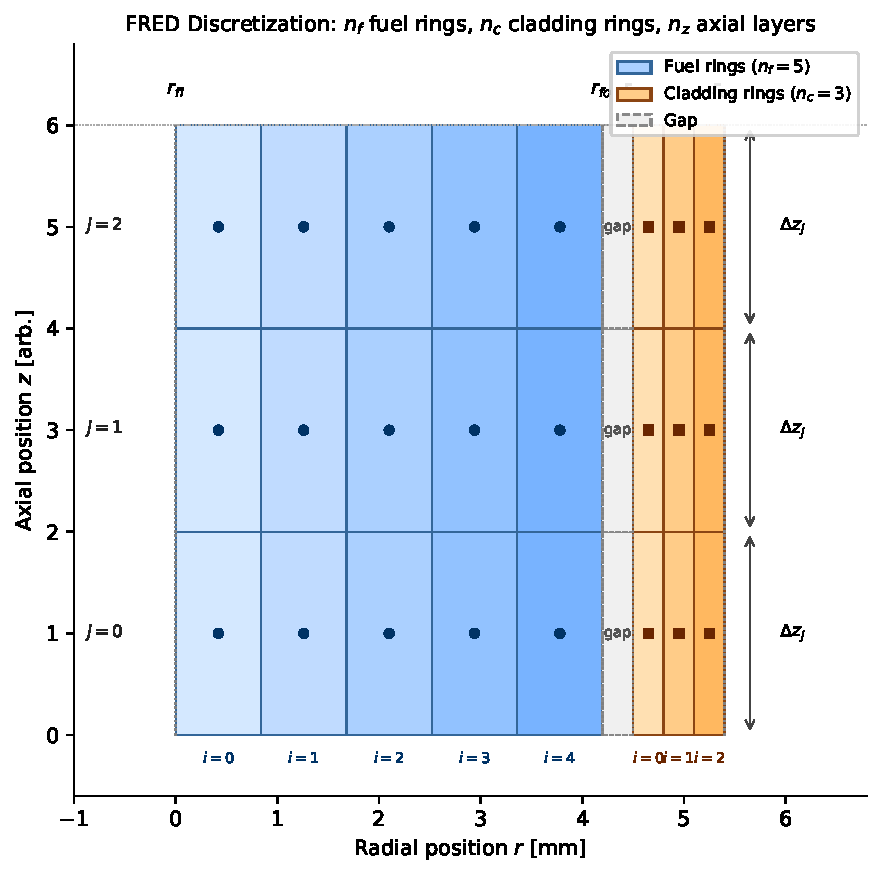
\includegraphics[width=0.85\textwidth]{images/rz_discretization.pdf}
  \caption{Schematic of the FRED radial-axial discretization.  The fuel pellet is divided into $n_f$ concentric rings (blue) and the cladding into $n_c$ rings (orange), separated by the fuel-cladding gap.  Each axial layer~$j$ has height~$\Delta z_j$.  Filled symbols denote the finite-volume node locations.}
  \label{fig:rz_discretization}
\end{figure}

\subsection{Governing Variables}

Table~\ref{tab:variables} lists the primary unknowns tracked at each axial layer and their governing equations.

\begin{table}[H]
  \centering
  \caption{Primary unknowns per axial layer in FRED.}
  \label{tab:variables}
  \begin{tabular}{llll}
    \toprule
    Symbol & Description & Units & Equation type \\
    \midrule
    $T_i$     & Temperature at radial node $i$ & K   & ODE \\
    $\sigma_r$, $\sigma_\theta$, $\sigma_z$ & Stress components & MPa & AE \\
    $\varepsilon_r$, $\varepsilon_\theta$, $\varepsilon_z$ & Strain components & - & AE \\
    $\delta$  & Gap width            & m   & AE \\
    $p_{fc}$  & Contact pressure     & MPa & AE \\
    $h_{gap}$ & Gap conductance      & W/(m$^2$\,K) & AE \\
    $p_{gas}$ & Internal gas pressure & MPa & AE  \\
    \bottomrule
  \end{tabular}
\end{table}

\printbibliography[heading=subbibliography,title={References}]
\end{refsection}

\clearpage

\begin{refsection}

\section{Thermal Conduction and Stress-Strain}
\label{sec:thermo_mech}

This section describes the core physics equations common to all FRED applications (FRED-ROD, FRED-OX, FRED-M-Na).  The equations are written first in differential (continuum) form and then in the finite-volume discretized form implemented in \texttt{HeatConduction.cpp} and \texttt{StressStrain.cpp}. It should be noted that the equations here present application agnostic equations, for example the correlation form of gap conductance, material property etc. are implemented in application specific code.

% =========================================================================
\subsection{Gap Pressure}
\label{sec:gap_pressure_rod}
% =========================================================================

The gap pressure $p_{gas}$ is a global algebraic variable common to all axial layers.  Two models are available, selected at the solver API level.

% -------------------------------------------------------------------------
\subsubsection{Prescribed Time-dependent Gap Pressure}
\label{sec:prescribed_pressure}
% -------------------------------------------------------------------------

The simplest model pins $p_{gas}$ to a user-supplied time series $p(t)$:
\begin{equation}
  p_{gas} = p(t).
  \label{eq:gpres_prescribed}
\end{equation}
The corresponding DAE residual is $r[0] = p_{gas} - p(t) = 0$.  A constant value is the most common case.

\paragraph{Typical use — liquid-bonded fuel.} In sodium-bonded metallic fuel (e.g.\ FRED-M-Na) the gap medium is liquid sodium.  Sodium is nearly incompressible, so the mechanical boundary condition at the cladding inner surface is set by the sodium \emph{system pressure}, not by a thermodynamic gas state.  The system pressure is approximately constant for a given operating condition and is prescribed directly via \texttt{set\_bond\_pressure(p\_MPa)}.

% -------------------------------------------------------------------------
\subsubsection{Gas Bond Pressure}
\label{sec:gas_bond_pressure}
% -------------------------------------------------------------------------

For gas-bonded fuel (e.g.\ He or Ar fill gas in FRED-ROD and FRED-OX) the pressure is determined by conservation of the molar fill-gas inventory $n$ under the ideal gas law:
\begin{equation}
  p_{gas} = \frac{n\,R}{v_T},
  \label{eq:gpres_ae}
\end{equation}
where $R = 8.314$~J/(mol\,K) is the universal gas constant.

\paragraph{Initial molar inventory.} The fill-gas moles are fixed from the as-fabricated conditions.  The user specifies the reference pressure $p_0$~[MPa] at room temperature $T_{ref} = 293.15$~K; together with the as-fabricated free volume $V_{free,0}$~[m$^3$] (gap annulus + central void + plenum),
\begin{equation}
  n = \frac{p_0 \times 10^6\; V_{free,0}}{R\,T_{ref}},
  \label{eq:mu0}
\end{equation}
and $n$ does not change during the simulation (no fission gas in FRED-ROD).

\paragraph{Temperature-weighted free volume.} The denominator $v_T$ is a temperature-weighted sum over all gas-filled regions:
\begin{multline}
  v_T = \frac{V_{pl}}{T_{pl}}
        + \sum_{j=0}^{n_z-1}
          \frac{\pi\,\Delta z_j\left(r_{ci,j}^2 - r_{fo,j}^2\right)}{T_{gap,j}} \\
        + \sum_{j=0}^{n_z-1}
          \frac{\pi\,\Delta z_j\,r_{fi,j}^2}{T_{ctr,j}}
  \label{eq:vT}
\end{multline}
where $V_{pl}$ is the plenum volume, $T_{pl}$ the plenum temperature, and $r_{fi,j}$, $r_{fo,j}$, $r_{ci,j}$ the deformed inner-fuel, outer-fuel, and inner-cladding radii of layer~$j$.  The central-void term vanishes for a solid pellet ($r_{fi,j} = 0$).

Two physical couplings follow directly from~\eqref{eq:gpres_ae}:
\begin{itemize}
\item \emph{Temperature rise} increases $v_T$ (larger $V/T$ terms) and therefore \emph{reduces} $p_{gas}$.
\item \emph{Gap closure} reduces the gap annulus volume, reducing $v_T$ and therefore \emph{increasing} $p_{gas}$ — which in turn raises the gas-pressure threshold that the contact pressure must exceed before the gap reopens.
\end{itemize}

\paragraph{FRED-OX.} In FRED-OX the molar inventory grows due to released fission gas: $n \to n + n_{fgr}(t)$, where $n_{fgr}$ is governed by its own ODE (Section~\ref{sec:fgr}).  Equation~\eqref{eq:gpres_ae} is otherwise identical; see Section~\ref{sec:gpres} for details.

% =========================================================================
\subsection{Thermal Conduction}
\label{sec:heat}
% =========================================================================

\subsubsection{Differential Form}

Assuming azimuthal symmetry, the transient heat conduction equation in cylindrical coordinates $(r,z)$ with volumetric heat generation $q'''$ is:

\begin{equation}
  \rho\, c_p \frac{\partial T}{\partial t}
  = \frac{1}{r}\frac{\partial}{\partial r}
    \!\left(r\,k\,\frac{\partial T}{\partial r}\right) + q'''
  \label{eq:heat_pde}
\end{equation}

where $\rho$ [kg/m$^3$] is the material density, $c_p$ [J/(kg\,K)] the isobaric heat capacity, $k$ [W/(m\,K)] the thermal conductivity, and $T$ [K] the temperature field.  Axial conduction is neglected in the current plane-strain implementation; each axial layer is solved independently.

\paragraph{Boundary conditions.}

\begin{itemize}
\item \emph{Symmetry at the fuel centre} (or inner hole gas pressure for annular pellets): $\partial T/\partial r = 0$ at $r = r_{fi}$ (solid pellet).
\item \emph{Fuel-cladding gap} at $r = r_{fo}$:
        \begin{equation}
          -k_f \frac{\partial T}{\partial r}\bigg|_{r_{fo}^-}
          = h_{gap}\,(T_f - T_c)
          \label{eq:gap_bc}
        \end{equation}
where $h_{gap}$ [W/(m$^2$\,K)] is the effective gap conductance (Section~\ref{sec:gap}) and $T_f, T_c$ are the fuel outer and cladding inner surface temperatures.
\item \emph{Coolant boundary} at $r = r_{co}$: two modes are available, reflecting the two principal use-cases for FRED.  In the first, FRED is coupled to an external sub-channel thermal-hydraulics (T-H) code that supplies the coolant temperature at all axial levels at all times; in the second, FRED uses in-built application sub-channel analysis and computes the coolant temperature internally.
        \begin{itemize}
\item \textbf{Dirichlet (prescribed temperature)} — FRED receives $T_{cool}(t)$ from the calling code or from a user-supplied time series and pins the outer cladding surface temperature directly:
                \begin{equation}
                  T\!\left(r_{co},t\right) = T_{cool}(t).
                  \label{eq:dirichlet_bc}
                \end{equation}
\item \textbf{Robin (convective HTC)} — a Newton's law of cooling condition is applied at the outer surface:
                \begin{equation}
                  -k_c\,\frac{\partial T}{\partial r}\bigg|_{r_{co}}
                  = h_{cool}(t)\,\bigl(T(r_{co},t) - T_{cool}(t)\bigr),
                  \label{eq:robin_bc}
                \end{equation}
where $h_{cool}$ [W/(m$^2$\,K)] is the cladding-to-coolant heat-transfer coefficient and $T_{cool}(t)$ is the \emph{local} bulk coolant temperature at the same axial position.  In the Robin mode both $h_{cool}$ and $T_{cool}$ are computed by an application-specific sub-channel model. Sub-channel variables (coolant properties, channel geometry, HTC correlation) are platform-specific; the FRED-M-Na sodium sub-channel implementation is described in Section~\ref{sec:subchannel_mna}.
        \end{itemize}
\end{itemize}

\subsubsection{Gap Conductance Model}
\label{sec:gap}

The thermal boundary condition at the fuel--cladding interface, Eq.~\eqref{eq:gap_bc}, requires an effective interfacial conductance $h_{gap}$. The physical form depends on whether the gap medium is a gas (free surface) or a liquid bond.

% ---- gas-filled gap ----
\paragraph{Gas-filled gap (free surface).} When the gap contains a cover gas (He, Ar, or a fission-gas/cover-gas mixture), the fuel outer surface is a \emph{free surface}: it carries only the normal gas pressure $p_{gas}$ and no tangential traction.  Heat transfer across the gas layer is limited by the low gas thermal conductivity and by a temperature discontinuity at each solid surface (temperature-jump effect).  The general form of the gas-gap conductance is:
\begin{equation}
  h_{gap}^{\mathrm{gas}} = \frac{k_{gas}(\bar{T})}{\delta + g_f + g_c} + h_{rad}
  \label{eq:hgap_gas}
\end{equation}
where
\begin{itemize}
\item $k_{gas}(\bar{T})$ is the gas thermal conductivity at mean gap temperature $\bar{T} = \tfrac{1}{2}(T_f + T_c)$,
\item $\delta = r_{ci} - r_{fo}$ is the physical gap width (Eq.~\eqref{eq:gap_ae}),
\item $g_f$ and $g_c$ are the temperature-jump distances at the fuel and cladding surfaces, accounting for partial accommodation of gas molecules at each wall, and
\item $h_{rad} = \sigma_{SB}\,\varepsilon_{\mathrm{eff}}\, (T_f^2 + T_c^2)(T_f + T_c)$ is the radiative contribution across the cavity, with $\sigma_{SB}$ the Stefan--Boltzmann constant and $\varepsilon_{\mathrm{eff}}$ the effective emissivity.
\end{itemize}
The gap pressure $p_{gas}$ is governed by the ideal-gas model (Section~\ref{sec:gas_bond_pressure}).  The variables $k_{gas}$, $g_f$, $g_c$, and $\varepsilon_{\mathrm{eff}}$ are application-specific correlations for example Section~\ref{sec:gap_ox} (FRED-OX).

% ---- liquid-filled gap ----
\paragraph{Liquid-filled gap.} When the gap is filled with a liquid bond (e.g.\ liquid sodium in FRED-M-Na), no temperature-jump effect because the liquid maintains continuous thermal contact with both solid surfaces.  The conductance reduces to:
\begin{equation}
  h_{gap}^{\mathrm{liq}} = \frac{k_{liq}(\bar{T})}{\delta}
  \label{eq:hgap_liq}
\end{equation}
where $k_{liq}(\bar{T})$ is the thermal conductivity of the liquid bond. Because $k_{\mathrm{Na}} \approx 60$--$80$\,W/(m\,K) at typical fast-reactor temperatures compared with $k_{\mathrm{He}} \approx 0.15$--$0.35$\,W/(m\,K) for helium, the liquid-bonded gap conductance is one to two orders of magnitude higher than a gas-bonded gap of equal width.

The mechanical boundary condition at a liquid-filled gap retains the same \emph{free-surface pressure} form as the gas case (open-gap conditions in Section~\ref{sec:stress_strain}).  Application-specific closures for $k_{liq}(\bar{T})$ are described in Section~\ref{sec:gap_mna} (FRED-M-Na).

\subsubsection{Finite-Volume Discretization}

The pellet cross-section is divided into $n_f$ concentric rings of uniform radial width $\Delta r_f = (r_{fo} - r_{fi})/(n_f - 1)$, and the cladding into $n_c$ rings of width $\Delta r_c = (r_{co} - r_{ci})/(n_c - 1)$.  Nodes are placed at ring centroids (vertex-centred scheme).

An energy balance over ring $i$ (cross-sectional area $A_i$ [m$^2$]) gives the ODE for fuel ring temperatures ($i = 0,\ldots,n_f - 1$):

\begin{equation}
  \rho_f c_{p,f}(T_i)\,A_i\,\frac{dT_i}{dt}
  = q'''\,A_i + Q_{i-1 \to i} - Q_{i \to i+1}
  \label{eq:heat_ode_fuel}
\end{equation}

and for inner cladding rings ($i = n_f,\ldots,n_f + n_c - 2$, no volumetric generation):

\begin{equation}
  \rho_c c_{p,c}(T_i)\,A_i\,\frac{dT_i}{dt}
  = Q_{i-1 \to i} - Q_{i \to i+1}
  \label{eq:heat_ode_clad}
\end{equation}

The inter-ring heat flow per unit axial length [W/m] between nodes $i$ and $i+1$ is evaluated using the interface-averaged conductivity at half-node radius $\bar{r}_i$:

\begin{equation}
  Q_{i \to i+1} = k\!\left(\tfrac{T_i + T_{i+1}}{2}\right)
                  \frac{T_i - T_{i+1}}{\Delta r} \cdot 2\pi\bar{r}_i
  \label{eq:Qflux}
\end{equation}

The outer cladding node carries an algebraic equation (AE) whose form depends on the active BC mode:

\begin{equation}
  \text{Dirichlet:}\quad T_{n_f+n_c-1} = T_{cool}(t)
  \label{eq:outerBC_dirichlet}
\end{equation}
\begin{equation}
  \text{Robin:}\quad Q_{n_f+n_c-2 \to n_f+n_c-1}
    = h_{cool}\cdot 2\pi r_{co}\cdot\bigl(T_{n_f+n_c-1} - T_{cool}(t)\bigr)
  \label{eq:outerBC_robin}
\end{equation}

In both cases the outer node equation is algebraic, so the equation count is unchanged.  The Robin form sets the conductive flux arriving at the outer ring equal to the convective flux leaving to the coolant; $h_{cool}$ and $T_{cool}$ are supplied by the application-specific sub-channel model.

The fuel-clad gap heat flow (index $i = n_f - 1$) is:
\begin{equation}
  Q_{gap} = h_{gap}\,(T_{n_f-1} - T_{n_f}) \cdot 2\pi r_{fo}
  \label{eq:Qgap}
\end{equation}

\paragraph{Auxiliary algebraic equations.} The DAE system carries four auxiliary scalar variables — volumetric power $q'''$, gap width $\delta$, contact pressure $p_{fc}$, and gap conductance $h_{gap}$ — each pinned by its own algebraic equation:
\begin{align}
  q'''    &= q'''(t)
            \label{eq:qqv_ae}\\
  \delta  &= r_{ci} - r_{fo}
            \label{eq:gap_ae}\\
  p_{fc}  &= \begin{cases}
               0                  & \text{(open gap)}   \\
               |\sigma_r^{(0)}|   & \text{(closed gap)}
             \end{cases}
            \label{eq:pfc_ae}\\
  h_{gap} &= h_{gap}(\,\cdot\,)
            \label{eq:hgap_ae}
\end{align}
where $r_{ci}$ and $r_{fo}$ are the deformed cladding inner and fuel outer radii, and $\sigma_r^{(0)}$ is the cladding inner surface radial stress. The gap conductance closure~\eqref{eq:hgap_ae} is application-specific (Section~\ref{sec:gap}).

\paragraph{Equation count.} The thermal block contributes $4 + n_f + n_c$ equations per axial layer:
\begin{itemize}
\item 4 auxiliary AEs: power density~\eqref{eq:qqv_ae}, gap width~\eqref{eq:gap_ae}, contact pressure~\eqref{eq:pfc_ae}, and gap conductance~\eqref{eq:hgap_ae}.
\item $n_f$ fuel temperature ODEs~\eqref{eq:heat_ode_fuel}.
\item $(n_c - 1)$ inner cladding temperature ODEs~\eqref{eq:heat_ode_clad}.
\item 1 outer cladding AE — either the Dirichlet form~\eqref{eq:outerBC_dirichlet} or the Robin form~\eqref{eq:outerBC_robin}; the equation count is the same for both modes.
\end{itemize}
The last two groups together give $n_c$ cladding equations, so the total is $4 + n_f + n_c$, regardless of which coolant BC is active.

The material thermal conductivity $k(T)$, heat capacity $c_p(T)$, and density $\rho$ formulations are application specific e.g. in FUEL-ROD, users can specify arbitrary correlations while in FRED-OX, correlations specific to MOX are used (~Section:\ref{sec:mox_correlations}).

% =========================================================================
\subsection{Stress-Strain}
\label{sec:stress_strain}
% =========================================================================

\subsubsection{Differential Form}

FRED applies the plane-strain / plane-stress assumption (all axial layers deform independently with a uniform axial strain $\varepsilon_z$), the governing equations for a cylindrical body in cylindrical coordinates $(r,\theta,z)$ are as follows:

\paragraph{Strain-displacement relations.}

In a thin circular ring of radius $r$ with radial displacement $u$. The radial strain a.k.a. the stretching of the ring in the radial direction is
\begin{equation}
  \varepsilon_r = \frac{du}{dr}.
\end{equation}

Taking a small arc length subtending an angle $d \theta$ of original length $ds = r d\theta$ and final lenght $ds' = (r + u) d \theta$, the strain of that arc is
\begin{equation}
  \varepsilon_\theta = \frac{ds' - ds}{ds} = \frac{(r + u)d \theta - r d\theta}{r d \theta} = \frac{u}{r}. 
\end{equation}

\begin{align}
  \varepsilon_\theta &= \frac{u}{r}, \quad
  \varepsilon_r = \frac{du}{dr}, \quad
  \varepsilon_z = \text{const (per layer)}
  \label{eq:strain_disp}
\end{align}

\paragraph{Radial compatibility.}
\begin{equation}
  \frac{d(r\,\varepsilon_\theta)}{dr} = \varepsilon_r
  \label{eq:compat_cont}
\end{equation}

\paragraph{Radial equilibrium.}
\begin{equation}
  \frac{d(r\,\sigma_r)}{dr} = \sigma_\theta
  \label{eq:equil_cont}
\end{equation}

\paragraph{Thermal strain.} The total strain is decomposed into elastic and thermal parts, $\varepsilon = \varepsilon^{el} + \varepsilon^{th}$, where the isotropic thermal expansion strain is
\begin{equation}
  \varepsilon^{th}(T) = \alpha_{\mathrm{CTE}}\,(T - T_{\mathrm{ref}})
  \label{eq:thermal_strain}
\end{equation}
with $\alpha_{\mathrm{CTE}}$ [1/K] the linear coefficient of thermal expansion and $T_{\mathrm{ref}}$ the stress-free reference temperature.

% Figure~\ref{fig:ring_compat_equil} gives an intuitive differential-ring view
% of these two constraints: non-uniform radial displacement across the ring
% enforces strain compatibility, while radial traction variation across the same
% ring enforces radial stress equilibrium.

% \begin{figure}[htbp]
%   \centering
%   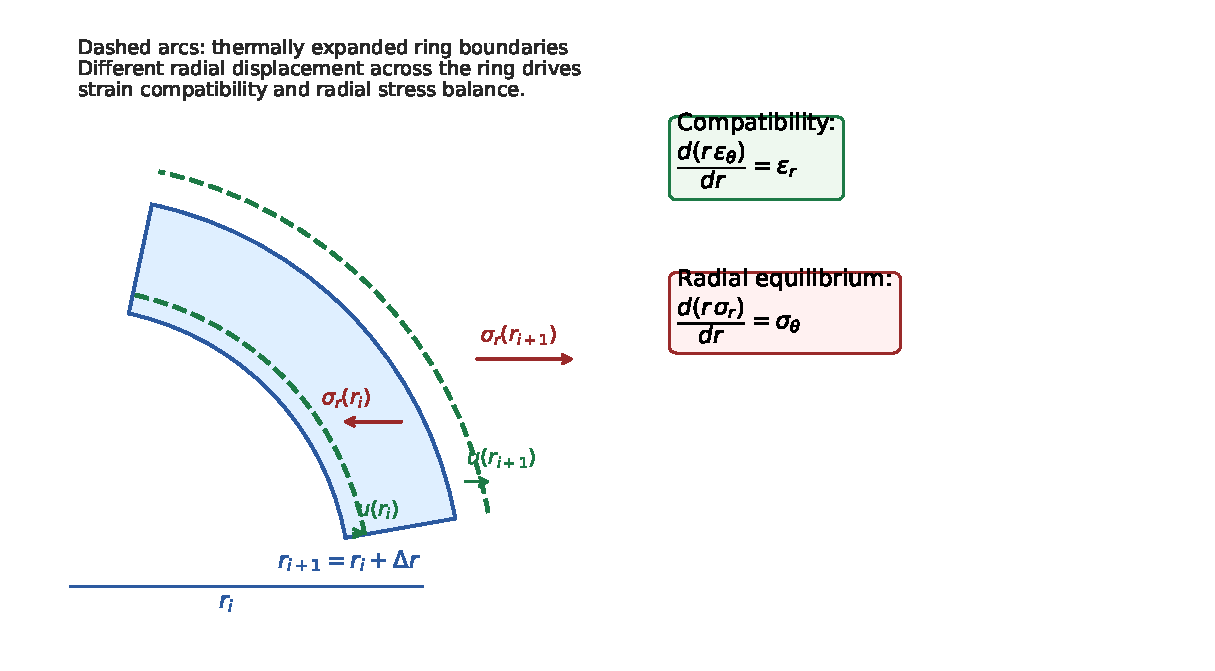
\includegraphics[width=0.90\textwidth]{images/mech_ring_compatibility.pdf}
%   \caption{Differential ring interpretation of radial strain compatibility and
%            radial stress equilibrium. Dashed arcs indicate differential thermal
%            expansion of inner/outer ring boundaries; radial traction arrows
%            indicate the balance represented by
%            $\frac{d(r\,\sigma_r)}{dr}=\sigma_\theta$.}
%   \label{fig:ring_compat_equil}
% \end{figure}

\paragraph{Thermo-elastic constitutive law (Hooke's law with thermal expansion).} Using the thermal strain~\eqref{eq:thermal_strain}, the elastic strains relate to stresses via:

\begin{align}
  E\,(\varepsilon_\theta - \varepsilon^{th}) &= \sigma_\theta - \nu(\sigma_r + \sigma_z)
  \label{eq:hooke_h}\\
  E\,(\varepsilon_r     - \varepsilon^{th}) &= \sigma_r     - \nu(\sigma_\theta + \sigma_z)
  \label{eq:hooke_r}\\
  E\,(\varepsilon_z     - \varepsilon^{th}) &= \sigma_z     - \nu(\sigma_\theta + \sigma_r)
  \label{eq:hooke_z}
\end{align}

where $E$ [MPa] is Young's modulus and $\nu$ Poisson's ratio.


\paragraph{Boundary conditions.}

Fuel (3 conditions) and cladding (3 conditions) each carry three boundary equations, giving six in total.

\emph{Fuel (BC-1, BC-2, BC-3):}
\begin{itemize}
\item \emph{BC-1 — Axial force balance}:
        \begin{itemize}
\item Open gap: $\displaystyle\sum_{i=0}^{n_f-1} A_{f,i}\,\sigma_{z,f}^{(i)} + A_{z,f}\,p_{gas} = 0$.
\item Closed gap (combined fuel+clad): $\displaystyle\sum_{i=0}^{n_f-1} A_{f,i}\,\sigma_{z,f}^{(i)} + \sum_{i=0}^{n_c-1} A_{c,i}\,\sigma_{z,c}^{(i)} + \pi r_{co}^2\,p_{cool} = 0$.
        \end{itemize}
\item \emph{BC-2 — Inner radial surface} (solid pellet): symmetry $\sigma_r^{(0)} = \sigma_\theta^{(0)}$.  For an annular pellet: $\sigma_r^{(0)} = -p_{gas}$.
\item \emph{BC-3 — Outer radial surface / gap interface}:
        \begin{itemize}
\item Open gap: $\sigma_r^{(n_f-1)} = -p_{gas}$.
\item Closed gap: axial strain compatibility $\varepsilon_z^{f} = \varepsilon_z^{c}$.
        \end{itemize}
\end{itemize}

\emph{Cladding (BC-1, BC-2, BC-3):}
\begin{itemize}
\item \emph{BC-1 — Axial / interface condition}:
        \begin{itemize}
\item Open gap (cladding axial force balance): $\displaystyle\sum_{i=0}^{n_c-1} A_{c,i}\,\sigma_{z,c}^{(i)} + \pi r_{co}^2\,p_{cool} - \pi r_{ci}^2\,p_{gas} = 0$.
\item Closed gap (radial traction continuity at fuel–clad interface): $\sigma_{r,f}^{(n_f-1)} = \sigma_{r,c}^{(0)}$.
        \end{itemize}
\item \emph{BC-2 — Inner radial surface}:
        \begin{itemize}
\item Open gap: $\sigma_r^{(0)} = -p_{gas}$.
\item Closed gap: gap width locked at surface roughness $\delta = \delta_{rough}$.
        \end{itemize}
\item \emph{BC-3 — Outer radial surface}: $\sigma_r^{(n_c-1)} = -p_{cool}$.
\end{itemize}

Here $A_{z,f} = \pi r_{fi}^2$ for annular fuel (zero for a solid pellet), so gas loading on the fuel end appears only when a central hole is present.
\label{eq:axial_balance}

\subsubsection{Finite-Volume Discretization}

Each ring~$i$ is treated as a finite-volume cell with area $A_i = \pi(r_{i+1}^2 - r_i^2)$.  The unknown strains and stresses are defined at the node location $r_i$.  The compatibility equation~\eqref{eq:compat_cont} integrated over a ring of width $\Delta r$ between nodes $i$ and $i+1$ gives:

\begin{equation}
  \Delta r\;\bar{\varepsilon}_r + r_i\,\varepsilon_\theta^{(i)}
  - r_{i+1}\,\varepsilon_\theta^{(i+1)} = 0
  \label{eq:compat_disc}
\end{equation}

where $\bar{\varepsilon}_r = \tfrac{1}{2}(\varepsilon_r^{(i)} + \varepsilon_r^{(i+1)})$.  The stress equilibrium equation \eqref{eq:equil_cont} over the same ring is:

\begin{equation}
  \Delta r\;\bar{\sigma}_\theta + r_i\,\sigma_r^{(i)}
  - r_{i+1}\,\sigma_r^{(i+1)} = 0
  \label{eq:equil_disc}
\end{equation}

with $\bar{\sigma}_\theta = \tfrac{1}{2}(\sigma_\theta^{(i)} + \sigma_\theta^{(i+1)})$.  At each node, the thermal expansion strain is also pinned to the local temperature by an algebraic equation,
\begin{equation}
  \varepsilon^{th}_i = \varepsilon^{th}(T_i),
  \label{eq:thexp_disc}
\end{equation}
where $\varepsilon^{th}(T)$ is defined in~\eqref{eq:thermal_strain}.  Together with the three Hooke's law equations~\eqref{eq:hooke_h}--\eqref{eq:hooke_z} and the boundary conditions listed above, each body with $n$ nodes contributes equations in three groups:
\begin{itemize}
\item $4n$ at-node equations: thermal expansion AE~\eqref{eq:thexp_disc} plus Hooke's law~\eqref{eq:hooke_h}--\eqref{eq:hooke_z} in $\theta$, $r$, $z$.
\item $2(n-1)$ inter-node equations: one compatibility~\eqref{eq:compat_disc} and one equilibrium~\eqref{eq:equil_disc} per adjacent node pair ($n-1$ pairs for $n$ nodes).
\item 3 boundary condition equations: inner radial surface, outer radial surface / gap interface, and axial force balance.
\end{itemize}
Each body therefore contributes $4n + 2(n-1) + 3 = 6n + 1$ equations. Summing fuel ($n = n_f$) and cladding ($n = n_c$):
\begin{equation}
  (6\,n_f + 1) + (6\,n_c + 1) = 6(n_f + n_c) + 2.
  \label{eq:mech_neq}
\end{equation}

\paragraph{Gap state machine.} The gap opens and closes as the fuel expands radially.  The event is detected by SUNDIALS IDA root-finding:

\begin{itemize}
\item \emph{Closure root}: $g_1 = \delta - \delta_{thresh} = 0$, $\delta_{thresh} = \rho_f + \rho_c$.
\item \emph{Reopening root}: $g_2 = p_{fc} - p_{gas} = 0$.
\end{itemize}

The closure root tracks the mechanical closure between the fuel pellet and the cladding, while the re-opening root tracks when the pressure in the gap exceeds the contact pressure, causing re-opening. Upon gap closure, the boundary-condition set switches as follows:

\begin{align}
  \text{Fuel outer BC (open)}\quad &\sigma_{r,f}^{(n_f-1)} = -p_{gas}
  \quad\Longrightarrow\quad
  \text{(closed)}\; \varepsilon_{z,f} - \varepsilon_{z,c} = 0 \\
  \text{Clad inner BC (open)}\quad &\sigma_{r,c}^{(0)} = -p_{gas}
  \quad\Longrightarrow\quad
  \text{(closed)}\; \delta - \delta_{rough} = 0
\end{align}

and the closed-gap contact interface additionally enforces radial traction continuity,
\begin{equation}
  \sigma_{r,f}^{(n_f-1)} - \sigma_{r,c}^{(0)} = 0.
\end{equation}

In the axial force balance, the branch switch is explicit:
\begin{itemize}
\item \emph{Open gap} (separate fuel and clad axial equilibrium):
        \begin{align}
          \sum_{i=0}^{n_f-1} A_{f,i}\,\sigma_{z,f}^{(i)} + A_{z,f}\,p_{gas} &= 0, \\
          \sum_{i=0}^{n_c-1} A_{c,i}\,\sigma_{z,c}^{(i)}
          + \pi r_{co}^2\,p_{cool} - \pi r_{ci}^2\,p_{gas} &= 0.
        \end{align}
\item \emph{Closed gap} (shared fuel+clad axial equilibrium):
        \begin{equation}
          \sum_{i=0}^{n_f-1} A_{f,i}\,\sigma_{z,f}^{(i)}
          + \sum_{i=0}^{n_c-1} A_{c,i}\,\sigma_{z,c}^{(i)}
          + \pi r_{co}^2\,p_{cool} = 0.
        \end{equation}
\end{itemize}
Here $A_{z,f}=\pi r_{fi}^2$ for annular fuel (and $A_{z,f}=0$ for a solid pellet), so gas loading on the fuel axial end appears only when a central hole exists.

\paragraph{Equation-of-state summary.} Including the one global gas-pressure AE~\eqref{eq:gpres_ae} and the per-layer thermal and mechanical blocks, the total equation count is
\begin{multline}
  \underbrace{1}_{\text{global }p_{gas}}
  \;+\;
  n_z\!\left[
    \underbrace{(4 + n_f + n_c)}_{\text{thermal}}
    +\;
    \underbrace{6(n_f + n_c) + 2}_{\text{mechanical}}
  \right] \\
  =\; 1 + n_z\bigl[7(n_f + n_c) + 6\bigr]
  \;\equiv\; 7(n_f + n_c) + 7 \;\text{(per layer + global).}
  \label{eq:neq_total}
\end{multline}

The state vector is ordered as follows:
\begin{equation}
  \mathbf{y} =
  \left[
  \begin{array}{cl}
    p_{gas}
      & \text{1 global AE~\eqref{eq:gpres_ae}} \\[4pt]
    \hline \\[-7pt]
    q'''_0,\;\delta_0,\;p_{fc,0},\;h_{gap,0}
      & \text{layer 0: 4 thermal AEs~\eqref{eq:qqv_ae}--\eqref{eq:hgap_ae}} \\
    T^{(0)}_0,\;\ldots,\;T^{(0)}_{n_f+n_c-1}
      & \text{layer 0: $n_f+n_c$ temperatures~\eqref{eq:heat_ode_fuel}--\eqref{eq:outerBC_dirichlet}} \\
    \varepsilon^{th}_{f,0},\ldots,\varepsilon^{h}_{f,0},\ldots,\varepsilon_{fz},\,
    \sigma^{h}_{f,0},\ldots
      & \text{layer 0: fuel mechanics ($6n_f+1$)} \\
    \varepsilon^{th}_{c,0},\ldots,\varepsilon^{h}_{c,0},\ldots,\varepsilon_{cz},\,
    \sigma^{h}_{c,0},\ldots
      & \text{layer 0: clad mechanics ($6n_c+1$)} \\[4pt]
    \hline \\[-7pt]
    \multicolumn{2}{c}{\vdots} \\[4pt]
    \hline \\[-7pt]
    q'''_{n_z-1},\;\delta_{n_z-1},\;\ldots
      & \text{layer $n_z-1$: (same structure)}
  \end{array}
  \right]
  \label{eq:state_vec}
\end{equation}

\printbibliography[heading=subbibliography,title={References}]
\end{refsection}

\clearpage

\begin{refsection}

\section{Time Integration: SUNDIALS IDA Solver}
\label{sec:sundials}

Time evolution of the fuel pin state in FRED-ROD and FRED-OX is delegated to SUNDIALS\,7.1.1 \cite{hindmarsh2005}, specifically to the IDA (Implicit Differential-Algebraic) solver component. FRED-M-Na is the one exception: it does not call SUNDIALS IDA at all, and instead implements its own fixed-step, always-accept backward-Euler driver to replicate a behaviour of the legacy Fortran reference code that IDA's adaptive step-acceptance logic cannot express; see Section~\ref{sec:mna_time_integration} for the details and the reasoning behind the departure.  Everything in the remainder of this chapter (Sections~\ref{sec:dae_formulation}--\ref{sec:error_diagnosis}) describes the SUNDIALS-IDA path used by FRED-ROD and FRED-OX. This chapter is structured as follows.  Section~\ref{sec:dae_formulation} introduces the mathematical form of the problem and describes how the FRED 2.0 solution vector is organised.  Section~\ref{sec:ida_algorithm} describes the IDA algorithm: the BDF time-integration scheme, the Newton nonlinear solver, and the error-control strategy.  Section~\ref{sec:calcic} documents consistent initial condition calculation.

Section~\ref{sec:root_finding} describes IDA's root-finding capability and how FRED 2.0 exploits it for discrete events.  Section~\ref{sec:gap_events} covers gap contact-state transitions in detail.  Section~\ref{sec:tolerances_fred2} discusses tolerance selection.  Section~\ref{sec:error_diagnosis} is a reference for IDA return codes and common failure modes.


%--------------------------------------------------------------------------------------------------
\subsection{Differential-Algebraic Formulation}
\label{sec:dae_formulation}
%--------------------------------------------------------------------------------------------------

\subsubsection{Residual Form}

The physical state of a fuel pin at time $t$ is packed as a state vector $\mathbf{y}(t) \in \mathbb{R}^N$ and $\dot{\mathbf{y}}(t) = \mathrm{d}\mathbf{y}/\mathrm{d}t$. IDA does not receive equations in solved form; it is given a residual function $F : \mathbb{R} \times \mathbb{R}^N \times \mathbb{R}^N \to \mathbb{R}^N$ and advances the solution by enforcing
\begin{equation}
  F\!\left(t,\,\mathbf{y}(t),\,\dot{\mathbf{y}}(t)\right) = \mathbf{0},
  \qquad t \in [t_0,\, t_\mathrm{end}].
  \label{eq:dae_general}
\end{equation}

Scalar equations $r_k = 0$ fall into two categories:
\begin{description}
\item[Ordinary differential equations (ODEs)] $r_k = \dot{y}_k - g_k(t,\mathbf{y}) = 0$, where $\dot{y}_k$ appears explicitly.  The associated variable $y_k$ is a \emph{differential variable} (IDA type identifier $\mathtt{id}_k = 1$).
\item[Algebraic constraints (AEs)] $r_k = h_k(t,\mathbf{y}) = 0$, where no time derivative appears.  The associated variable $y_k$ is an \emph{algebraic variable} ($\mathtt{id}_k = 0$).
\end{description}

The arrangement of the solution vector is application specific and is detailed more in the developer guide.

%------------------
\subsection{The IDA Algorithm}
\label{sec:ida_algorithm}
%------------------

\subsubsection{Backward Differentiation Formula}
\label{subsec:bdf}

IDA advances the solution using a variable-order, variable-step Backward Differentiation Formula (BDF)~\cite{hindmarsh2005}.  The BDF method of order~$q$ approximates the time derivative at $t_n$ as a linear combination of the current and $q$ most recently accepted solution values:
\begin{equation}
  \dot{\mathbf{y}}_n \approx \frac{1}{h_n}\sum_{i=0}^{q}\alpha_{q,i}\,\mathbf{y}_{n-i},
  \label{eq:bdf}
\end{equation}
where $h_n = t_n - t_{n-1}$ is the current step size and $\alpha_{q,i}$ are the BDF coefficients determined by the order~$q$.

Substituting~\eqref{eq:bdf} into~\eqref{eq:dae_general} gives the nonlinear corrector equation to be solved at each step:
\begin{equation}
  G(\mathbf{y}_n) \equiv
  F\!\!\left(t_n,\,\mathbf{y}_n,\,
    \frac{1}{h_n}\sum_{i=0}^{q}\alpha_{q,i}\,\mathbf{y}_{n-i}\right) = \mathbf{0}.
  \label{eq:corrector}
\end{equation}

The BDF order $q$ ranges from 1 to 5.  The solver starts at order~1 (backward Euler, BE) and dynamically increases the order when doing so allows a larger step size while still satisfying the local truncation error test.  For $q=1$:
\begin{equation}
  \dot{\mathbf{y}}_n \approx \frac{\mathbf{y}_n - \mathbf{y}_{n-1}}{h_n},
  \label{eq:be}
\end{equation}
which is the scheme applied on the very first time step.

\subsubsection{Predictor--Corrector Cycle}

At each step, IDA executes a predictor--corrector cycle.

\paragraph{BDF predictor.} Using the Nordsieck history array built from the $q$ most recently accepted steps, IDA extrapolates the predicted state at $t_n$:
\begin{equation}
  \mathbf{y}_n^{(0)} = \sum_{i=0}^{q} A_{q,i}\,\mathbf{y}_{n-i},
  \qquad
  \dot{\mathbf{y}}_n^{(0)} = \dot{\mathbf{y}}_{n-1}
    + \frac{\alpha_{q,0}}{h_n}\bigl(\mathbf{y}_n^{(0)} - \mathbf{y}_{n-1}^{(0)}\bigr),
  \label{eq:predictor}
\end{equation}
where $A_{q,i}$ are the BDF extrapolation coefficients and $\alpha_{q,0}$ is the leading BDF coefficient.

\paragraph{Newton corrector.} Starting from the predicted state $\mathbf{y}_n^{(0)}$, IDA iterates:
\begin{equation}
  J^{(m)}\,\delta\mathbf{y}^{(m)} = -G\!\left(\mathbf{y}_n^{(m)}\right),
  \qquad
  \mathbf{y}_n^{(m+1)} = \mathbf{y}_n^{(m)} + \delta\mathbf{y}^{(m)},
  \label{eq:newton}
\end{equation}
where the \emph{IDA iteration matrix} is
\begin{equation}
  J = \frac{\partial F}{\partial \mathbf{y}}
    + c_J\,\frac{\partial F}{\partial \dot{\mathbf{y}}},
  \qquad
  c_J = \frac{\alpha_{q,0}}{h_n}.
  \label{eq:jacobian}
\end{equation}
At each Newton iterate the time derivative is updated via the BDF consistency relation:
\begin{equation}
  \dot{\mathbf{y}}_n^{(m)} = \dot{\mathbf{y}}_n^{(0)}
    + \frac{\alpha_{q,0}}{h_n}\bigl(\mathbf{y}_n^{(m)} - \mathbf{y}_n^{(0)}\bigr).
  \label{eq:ydot_update}
\end{equation}

The factor $c_J$ in~\eqref{eq:jacobian} enters because perturbing $y_k$ by $\delta$ during the Jacobian build simultaneously perturbs $\dot{y}_k$ by $c_J\delta$ through the BDF consistency relation.  For an ODE residual $r_i = \dot{y}_i - g_i(t,\mathbf{y})$, the diagonal Jacobian entry is $J_{ii} = c_J - \partial g_i/\partial y_i$.  For an algebraic residual $r_i = h_i(t,\mathbf{y})$, the $c_J$ term does not appear.

FRED 2.0 does not supply an analytic Jacobian.  IDA approximates $J$ internally using finite-difference perturbations of the residual function, perturbing each column $j$ as
\begin{equation}
  J_{:,j} \approx
    \frac{F\!\left(t,\,\mathbf{y}+\delta_j\mathbf{e}_j,\,
                    \dot{\mathbf{y}}+c_J\delta_j\mathbf{e}_j\right)
          - F(t,\mathbf{y},\dot{\mathbf{y}})}{\delta_j},
  \qquad
  \delta_j = \sqrt{\varepsilon_\mathrm{mach}}\,\max\!\bigl(|y_j|,\,10^{-6}\bigr),
  \label{eq:fd_jacobian}
\end{equation}
where the simultaneous perturbation of $\dot{\mathbf{y}}$ by $c_J\delta_j$ follows from the BDF consistency relation~\eqref{eq:ydot_update}.

\paragraph{Newton convergence criterion.} Newton iteration is declared converged when the weighted root-mean-square (WRMS) norm of the Newton correction satisfies
\begin{equation}
  \bigl\|\delta\mathbf{y}^{(m)}\bigr\|_\mathrm{WRMS} < 0.33,
  \label{eq:newton_conv}
\end{equation}
where the WRMS norm with per-component tolerance weights $w_k$ is
\begin{equation}
  \|\mathbf{v}\|_\mathrm{WRMS}
  = \sqrt{\frac{1}{N}\sum_{k=1}^{N}\left(\frac{v_k}{w_k}\right)^{\!2}},
  \qquad
  w_k = \mathtt{rtol}\cdot|y_k| + \mathtt{atol}_k.
  \label{eq:wrms}
\end{equation}

\paragraph{Failure modes and step-size recovery.} A step is rejected and IDA retries with a reduced step size ($h \leftarrow h/4$) for three reasons:
\begin{enumerate}
\item \textbf{Jacobian ill-posed.}  LU factorisation of $J$ fails (singular or near-singular matrix); Newton aborts immediately.
\item \textbf{Newton non-convergence.}  The WRMS norm~\eqref{eq:newton_conv} fails to satisfy the convergence criterion within \texttt{IDASetMaxNonlinIters} iterations (default: 4).  IDA halves $h$ and rebuilds the Jacobian before retrying.
\item \textbf{Non-physical geometry.}  If swelling or creep increments drive a geometric quantity (node radius, ring thickness, axial layer height) to a non-positive value, \texttt{FuelRodState::\allowbreak{}updateGeometry} flags the condition.  The resulting residuals are extremely large or ill-defined, preventing Newton convergence.  IDA reduces $h$ and retries; if $h$ falls below $h_\mathrm{min}$, IDA aborts with \texttt{IDA\_ERR\_FAIL} (Section~\ref{sec:error_diagnosis}).
\end{enumerate}

\subsubsection{Step-Size and Order Control}
\label{subsec:step_control}

\paragraph{Local truncation error test.} After a successful Newton solve, IDA estimates the local truncation error (LTE) vector $\mathbf{e}_n$, which is proportional to the Newton correction relative to the predictor.

The step is accepted only if
\begin{equation}
  \|\mathbf{e}_n\|_\mathrm{WRMS} \leq 1.
  \label{eq:lte_test}
\end{equation}
Algebraic variables ($\mathtt{id}_k = 0$) are excluded from this norm via \texttt{IDASetSuppressAlg}, because their LTE estimate is $\mathcal{O}(1)$ and independent of $h_n$.

If the error test fails, the step size is reduced as
\begin{equation}
  h_\mathrm{new} = h_n \cdot \min\!\left(0.9,\;
    \|\mathbf{e}_n\|_\mathrm{WRMS}^{-1/(q+1)}\right),
  \label{eq:hreduce}
\end{equation}
and the corrector step is repeated.  If the error test fails more than \texttt{IDASetMaxErrTestFails} times in succession (default: 10), or if $h_n$ falls below the internal minimum $h_\mathrm{min}$, IDA aborts with \texttt{IDA\_ERR\_FAIL}.

\paragraph{Minimum step size.} IDA enforces an internal minimum step size
\begin{equation}
  h_\mathrm{min} = \varepsilon_\mathrm{mach} \cdot t_n,
  \label{eq:hmin}
\end{equation}
where $\varepsilon_\mathrm{mach} \approx 2.22 \times 10^{-16}$ is IEEE-754 double-precision machine epsilon. At early times $t_n \approx 0$ this floor approaches zero; in practice SUNDIALS imposes a floor around $10^{-6}$--$10^{-5}$\,s to prevent infinite halving.

\paragraph{Order selection.} At each accepted step, IDA evaluates whether increasing or decreasing $q$ by one would permit a larger step size while still satisfying~\eqref{eq:lte_test}.  The order is selected to maximise $h_n$ subject to the LTE test, up to the maximum order of~5.

\paragraph{Maximum step size.} FRED 2.0 does not enforce an explicit maximum step size.  The step size grows adaptively until limited by the error test or the requested output time.

%--------------------------------------------------------------------------------------------------
\subsection{Root-Finding and Solver Restarts}
\label{sec:root_finding}
%--------------------------------------------------------------------------------------------------

During time integration IDA continuously monitors user-supplied scalar indicator functions
\begin{equation}
  g_i\!\left(t,\,\mathbf{y}(t),\,\dot{\mathbf{y}}(t)\right), \quad i = 1,\ldots,n_r,
  \label{eq:root_fns}
\end{equation}
and locates their zero crossings to machine precision using a modified Illinois algorithm~\cite{hindmarsh2005}. When any $g_i$ changes sign during a step, IDA halts, returns \texttt{IDA\_ROOT\_RETURN}, and records which indicators changed sign. The caller inspects the event, updates any discontinuous model state, and---if the residual branch structure has changed---calls \texttt{IDAReInit} to flush the BDF Nordsieck history to order~1, allowing the integrator to restart cleanly on the updated residual branch.

\paragraph{Gap contact-state transitions.} FRED 2.0 exploits this mechanism to detect discrete fuel--cladding contact events. One root function per axial layer monitors the gap width (open-gap regime) or the gas-pressure--contact-pressure difference (closed-gap regime). When a sign change is detected, FRED switches branch logic and performs a structural restart so that IDA rebuilds its BDF history against the updated residual. The root functions, event handlers, and restart procedure are described in Section~\ref{sec:gap_events}.

\paragraph{Non-physical geometry.} Swelling or creep increments that are too large can drive geometric quantities---node radii, ring thicknesses, or axial layer heights---below zero. \texttt{FuelRodState::\allowbreak{}updateGeometry} computes updated geometry from the current strain state and returns \texttt{false} when any such quantity is non-positive. Because residuals depend on these geometric quantities (cross-sectional areas, heat-flux radii, contact surfaces), a non-physical geometry produces residuals that are extremely large or ill-defined. Newton iteration then fails to converge within the allowed number of steps, and IDA responds by halving the step size and retrying with a fresh Jacobian. If the step size falls below $h_\mathrm{min} \approx \varepsilon_\mathrm{mach} \cdot t_n$, IDA aborts with \texttt{IDA\_ERR\_FAIL}. In practice the adaptive step-size control keeps time steps small enough that geometric quantities remain positive throughout the run.


%--------------
\subsection{Consistent Initial Conditions}
\label{sec:calcic}
%--------------

IDA requires that $F(t_0, \mathbf{y}_0, \dot{\mathbf{y}}_0) = \mathbf{0}$ before the first step.  The algebraic components of $\mathbf{y}_0$ (gap width, contact pressure, gap conductance, power density, stresses, etc.) must be mutually consistent with the differential components (temperatures, burnup, swelling strains) at $t = t_0$.  Since $\dot{\mathbf{y}}_0$ cannot in general be prescribed analytically, FRED 2.0 uses the SUNDIALS routine \texttt{IDACalcIC} with mode \texttt{IDA\_YA\_YDP\_INIT}, which:

\begin{enumerate}
\item holds the differential variables $\mathbf{y}_d$ (those with $\mathtt{id}_k = 1$) fixed at their initial values,
\item simultaneously solves for the consistent algebraic variables $\mathbf{y}_a$ ($\mathtt{id}_k = 0$) and the initial derivatives $\dot{\mathbf{y}}_d(t_0)$ that satisfy~\eqref{eq:dae_general}.
\end{enumerate}

For example, the heat-equation residual for fuel node $i$ at axial layer $j$ is
\begin{equation}
  r_{T,i,j} =
    \rho_f c_{p,f} A_i \dot{T}_{i,j}
    - q_{v,j}^{\prime\prime\prime} A_i
    + q_{i}(t_0)\,2\pi r_i^0
    - q_{i-1}(t_0)\,2\pi r_{i-1}^0 = 0,
\end{equation}
so that \texttt{IDACalcIC} finds the consistent initial temperature time derivative
\begin{equation}
  \dot{T}_{i,j}(t_0)
  = \frac{q_{v,j}^{\prime\prime\prime}(t_0)\,A_i
          - q_{i}(t_0)\,2\pi r_i^0
          + q_{i-1}(t_0)\,2\pi r_{i-1}^0}
         {\rho_f c_{p,f} A_i}.
\end{equation}
For purely algebraic constraints (e.g. gap conductance, contact pressure, stresses), the condition simply requires $h_k(t_0, \mathbf{y}_0) = 0$.  The implementation details of \texttt{IDACalcIC} within \texttt{FredSolverBase} are documented in the Developer Guide.

%----------------
\subsection{Gap Event Detection and Structural Restart}
\label{sec:gap_events}
%----------------

\subsubsection{Root-Finding for Contact-State Transitions}

FRED 2.0 uses IDA's built-in root-finding capability to detect discrete fuel--cladding gap contact transitions during time integration. For each axial layer $j = 1, \ldots, n_z$, a single root function $g_j(t)$ is registered. The root function is normalised and changes form depending on the current contact state to make both closure and reopening detectable as sign changes:

\begin{equation}
  g_j(t) = \begin{cases}
    \dfrac{\delta_j(t) - \delta_\mathrm{contact}}{\delta_\mathrm{contact}}
      & \text{if gap is open} \\[10pt]
    \dfrac{p_\mathrm{gas}(t) - p_{\mathrm{fc},j}(t)}{p_{\mathrm{fc},j}(t) + p_\mathrm{gas}(t) + \varepsilon}
      & \text{if gap is closed,}
  \end{cases}
  \label{eq:root_function}
\end{equation}
where $\delta_\mathrm{contact} = \delta_\mathrm{ruff} + \delta_\mathrm{rufc}$ is the combined roughness contact threshold, $p_\mathrm{gas}$ is the plenum gas pressure, and $\varepsilon = 10^{-10}$ prevents division by zero. The normalisation keeps $g_j$ dimensionless and $\mathcal{O}(1)$ near the crossing, which is important for IDA's internal bisection algorithm.

\paragraph{Gap closure.} While the gap is open, $g_j > 0$. As the fuel thermally expands and the geometric clearance $\delta_j$ falls toward $\delta_\mathrm{contact}$, $g_j$ decreases monotonically through zero. IDA reports this as a \emph{falling} crossing; the contact state is switched to closed and a structural restart is performed.

\paragraph{Gap reopening.} While the gap is closed, $g_j < 0$ (gas pressure is less than contact pressure). As $p_{\mathrm{fc},j}$ decays (e.g.\ after a power reduction), $g_j$ rises through zero. IDA reports this as a \emph{rising} crossing; the contact state is switched to open and a structural restart is performed.

\paragraph{Why the contact-state flag is the branch selector.} During IDA's internal Newton iterations, the contact pressure $p_{\mathrm{fc},j}$ is a trial value that may be anywhere on the solution manifold. Using $p_{\mathrm{fc},j} < \varepsilon$ as a branch selector would cause $g_j$ to change form inside a single bisection interval, breaking IDA's sign-change bracket. The contact-state flag is only updated by the event handler (after \texttt{IDASolve} returns \texttt{IDA\_ROOT\_RETURN}), so the root function~\eqref{eq:root_function} is consistent throughout every bisection sweep for each IDA step.

\begin{table}[H]
  \centering
  \caption{Root-function sign convention for gap contact-state events.
           The bracket sign \texttt{glo[j]} at the left endpoint of the bisection interval
           determines the reported crossing direction.}
  \label{tab:root_signs}
  \begin{tabular}{lp{3cm}p{3cm}p{2.5cm}p{3cm}}
    \toprule
    Event & Active branch & $g_j$ motion & \texttt{rootsfound} & State change \\
    \midrule
    Closure   & gap open & $+\to 0^-$ (falling) & $-1$ & open $\to$ closed \\
    Reopening & gap closed & $-\to 0^+$ (rising)  & $+1$ & closed $\to$ open \\
    \bottomrule
  \end{tabular}
\end{table}

\subsubsection{Fixed-Time Forcing Roots}

In addition to the $n_z$ gap-state root functions, FRED applications can register $n_\mathrm{fix}$ forced stop-time root functions
\begin{equation}
  g_{n_z + k}(t) = t - t_{\mathrm{fix},k}, \qquad k = 1,\ldots,n_\mathrm{fix},
  \label{eq:fixed_time_roots}
\end{equation}
where $t_{\mathrm{fix},k}$ are user-specified times. These always cross from negative to positive (\texttt{rootsfound} $= +1$) and do not trigger any gap-state update. Their purpose is to force IDA to stop and restart exactly at the specified time, re-establishing the BDF history on a clean temporal boundary --- useful for capturing known transients or power changes that would otherwise be straddled by a large adaptive step.

\subsubsection{Structural Restart After an Event}

Discrete contact transitions change the algebraic regime of the DAE: the residual branch switches between the open-gap and closed-gap formulations. Continuing with a multistep BDF history built for the pre-event branch would degrade convergence and robustness. FRED therefore performs a structural restart at every event:

\begin{enumerate}
\item \textbf{Query event channels} --- inspect which root functions changed sign and update the contact-state flags.
\item \textbf{Reinitialise the solver} --- call \texttt{IDAReInit} at the event time $t_\mathrm{event}$ to flush the Nordsieck history and reset to BDF order~1.
\item \textbf{Restore DAE consistency} --- call \texttt{IDACalcIC} with mode \texttt{IDA\_YA\_YDP\_INIT} to solve for the consistent algebraic variables and initial derivatives on the new residual branch.
\item \textbf{Resume integration} --- continue from $t_\mathrm{event}$ on the updated branch.
\end{enumerate}

The contact-state flag must only be modified in the event dispatch loop (after \texttt{IDASolve} returns \texttt{IDA\_ROOT\_RETURN}), never inside the residual or root-function callbacks. IDA invokes these callbacks an unbounded number of times per step, including with speculative trial values; any premature mutation of the contact-state flag permanently corrupts the branch logic for subsequent Newton iterations. The implementation details --- event handlers, sign conventions, and failure-handling policy --- are documented in the Developer Guide.

%-------------------
\subsection{Tolerances}
\label{sec:tolerances_fred2}
%-------------------

IDA uses a mixed absolute/relative tolerance scheme.  For each component $k$ the effective tolerance weight is
\begin{equation}
  w_k = \mathtt{rtol} \cdot |y_k| + \mathtt{atol}_k,
\end{equation}
and both the Newton convergence test~\eqref{eq:newton_conv} and the LTE test~\eqref{eq:lte_test} use the WRMS norm~\eqref{eq:wrms}.

In FRED 2.0, a single scalar \texttt{rtol} and a single scalar \texttt{atol} (broadcast to all components) are set via \texttt{FredSolverBase::setTolerances}.  Recommended values for production runs are $\mathtt{rtol} = 10^{-5}$ and $\mathtt{atol} = 10^{-7}$.  Tighter tolerances increase accuracy at the cost of smaller step sizes and longer run times. If \texttt{IDACalcIC} fails at $t = 0$, try loosening both tolerances.

%-------------------
\subsection{Error Diagnosis and Troubleshooting}
\label{sec:error_diagnosis}
%-------------------

\subsubsection{Return Codes from \texttt{IDASolve}}

Table~\ref{tab:retval} lists all IDA return codes that can be emitted by \texttt{IDASolve}.

\begin{longtable}{p{1.2cm}p{5cm}p{7.5cm}}
  \toprule
  Code & Constant & Meaning \\
  \midrule
  \endhead
  $+2$  & \texttt{IDA\_ROOT\_RETURN}      & A root was found (gap closure, reopening, or fixed time). Execution continues. \\
  $+1$  & \texttt{IDA\_TSTOP\_RETURN}     & The solver reached the stop time set by \texttt{IDASetStopTime}. \\
  $0$   & \texttt{IDA\_SUCCESS}           & Normal return; the requested output time was reached. \\
  $-1$  & \texttt{IDA\_TOO\_MUCH\_WORK}   & More than \texttt{IDASetMaxNumSteps} internal steps taken without reaching the output time. \\
  $-2$  & \texttt{IDA\_TOO\_MUCH\_ACC}    & Tolerances are too tight for double-precision arithmetic. \\
  $-3$  & \texttt{IDA\_ERR\_FAIL}         & Error test failed \texttt{IDASetMaxErrTestFails} times in succession, or $h$ reached $h_\mathrm{min}$ without passing. \\
  $-4$  & \texttt{IDA\_CONV\_FAIL}        & Newton iteration failed to converge after excessive step-size reductions. \\
  $-5$  & \texttt{IDA\_LINIT\_FAIL}       & Linear solver initialisation failed. \\
  $-6$  & \texttt{IDA\_LSETUP\_FAIL}      & Jacobian evaluation or LU factorisation failed. \\
  $-7$  & \texttt{IDA\_LSOLVE\_FAIL}      & Back-substitution failed (singular pivot). \\
  $-8$  & \texttt{IDA\_RES\_FAIL}         & The residual function returned a non-recoverable error (return value $< 0$). \\
  $-9$  & \texttt{IDA\_REP\_RES\_ERR}     & The residual function returned a recoverable error ($= 1$) repeatedly. \\
  $-10$ & \texttt{IDA\_RTFUNC\_FAIL}      & The root-finding function returned a failure. \\
  $-12$ & \texttt{IDA\_FIRST\_RES\_FAIL}  & The residual function failed at the very first call ($t = t_0$). \\
  $-14$ & \texttt{IDA\_NO\_RECOVERY}      & The solver could not recover from a combination of failures. \\
  \bottomrule
  \caption{\texttt{IDASolve} return codes.}
  \label{tab:retval}
\end{longtable}

\subsubsection{\texttt{IDA\_ERR\_FAIL} (retval $= -3$): Error Test Failure}

\paragraph{What happened.} IDA proposed a step, solved the corrector, and evaluated the LTE estimate~\eqref{eq:lte_test}. The error test failed; the step size was halved repeatedly according to~\eqref{eq:hreduce}. After \texttt{IDASetMaxErrTestFails} consecutive failures (default: 10), or once $h$ reached $h_\mathrm{min}$~\eqref{eq:hmin}, IDA aborted.

\paragraph{Root causes.}
\begin{description}
\item[Inconsistent initial conditions (most common).] IDA requires $F(t_0,\mathbf{y}_0,\dot{\mathbf{y}}_0) = \mathbf{0}$ before the first step.  If $\mathbf{y}_0$ is not consistent with all algebraic constraints and ODEs, the residual is permanently non-zero at $t_0$ regardless of step size.
\item[Extreme stiffness.] Widely separated time scales at $t=0$ (fast thermal transients combined with slow creep) can make the Jacobian severely ill-conditioned, preventing Newton convergence at any step size.
\item[Tolerances inconsistent with problem scale.] If an absolute tolerance $\mathtt{atol}_k$ is much smaller than $|y_k|$ at $t_0$, the WRMS norm is dominated by that component and the error test becomes nearly impossible to satisfy.
\item[Non-physical initial state.] If material properties or geometry produce a residual that is ill-posed at $t_0$ (zero thermal conductivity, negative gap, etc.), the residual can return NaN or Inf.
\end{description}

\paragraph{Remedies.}
\begin{enumerate}
\item Check initial consistency by printing the residual vector at $t_0$ before the solver starts.
\item Temporarily loosen absolute tolerances and tighten progressively if the run succeeds.
\item Increase \texttt{IDASetMaxErrTestFails} to give the solver more attempts at small $h$.
\item Increase \texttt{IDASetMaxNonlinIters} when the Jacobian is poorly conditioned.
\item Verify that as-fabricated geometry is consistent (gap width equals cladding inner radius minus fuel outer radius).
\end{enumerate}

\subsubsection{\texttt{IDA\_TOO\_MUCH\_WORK} (retval $= -1$): Step Limit Exceeded}

The solver took more than \texttt{IDASetMaxNumSteps} internal steps between two consecutive output times. The physics are being integrated correctly but the output interval is too coarse relative to the required step size. Increase \texttt{IDASetMaxNumSteps} (e.g.\ to 5000).

\subsubsection{\texttt{IDA\_CONV\_FAIL} (retval $= -4$): Newton Convergence Failure}

Newton iteration did not converge within \texttt{IDASetMaxNonlinIters} iterations even after the step size was halved multiple times. This typically indicates:
\begin{itemize}
\item A nearly singular Jacobian at gap closure or when plasticity activates.
\item A near-discontinuity in the residual from a sudden power change or contact event not handled by a root function.
\item Material property correlations returning non-smooth values.
\end{itemize}
Increase \texttt{IDASetMaxNonlinIters}, or force the solver to stop and reinitialise exactly at the problematic time using a fixed-time root~\eqref{eq:fixed_time_roots}.

\subsubsection{\texttt{IDA\_LSOLVE\_FAIL} (retval $= -7$): Linear Solver Failure}

The dense LU factorisation of the Jacobian encountered a zero or near-zero pivot, indicating a numerically singular system matrix. In FRED 2.0 this can occur when:
\begin{itemize}
\item The contact state flag is inconsistent with the actual gap geometry, causing a conflict between open-gap and closed-gap residual branches.
\item A stress or strain variable is unconstrained due to a missing boundary condition.
\end{itemize}
Verify that the contact-state flags are consistent with the gap geometry at the time of failure.

\subsubsection{\texttt{IDA\_TOO\_MUCH\_ACC} (retval $= -2$): Accuracy Not Achievable}

The requested tolerances are tighter than double-precision arithmetic can provide. This typically manifests after many steps when accumulated round-off error dominates the LTE estimate. Loosen \texttt{rtol} (e.g.\ from $10^{-8}$ to $10^{-6}$) and the corresponding absolute tolerances.

\printbibliography[heading=subbibliography,title={References}]
\end{refsection}

\clearpage

\begin{refsection}

\section{Introduction}

FRED-OX is a refactored version of the FRED fuel performance code, originally developed by Konstantin Mikityuk and collaborators for the analysis of MOX fuel behaviour in sodium-cooled fast reactors.

If FRED-OX is used in scientific publications, please cite the following references.

\begin{verbatim}
@article{Mikityuk2011FRED,
  author    = {Konstantin Mikityuk and Andrei Shestopalov},
  title     = {FRED fuel behaviour code: Main models and
               analysis of Halden IFA-503.2 tests},
  journal   = {Nuclear Engineering and Design},
  year      = {2011},
  volume    = {241},
  number    = {7},
  pages     = {2455--2461},
  doi       = {10.1016/j.nucengdes.2011.04.033}
}

@inproceedings{Kriventsev2015TopFuel,
  author    = {Vladimir Kriventsev and Andrei Rineiski and Werner Pfrang and
               Sara Perez-Martin and Konstantin Mikityuk and
               Grigori Khvostov},
  title     = {Benchmark on Behavior of MOX Fuel Pin Under
               Irradiation at Nominal Power in Sodium Fast Reactor},
  booktitle = {Proceedings of TopFuel 2015},
  year      = {2015},
  address   = {Zurich, Switzerland}
}
\end{verbatim}

\section{Base Irradiation Physics: MOX Fuel and Cladding (FRED-OX)}
\label{sec:fred_ox}

FRED-OX extends the FRED-ROD thermo-mechanical solver with irradiation physics relevant to mixed oxide (Pu-U-O) fuel. The following additional variables and phenomena are introduced:

\begin{itemize}
\item \textbf{Burnup} $B$ [MWd/kgU]: volumetric energy deposited in the fuel; drives all irradiation-dependent property changes.
\item \textbf{Fission gas generation and release} $\mu_{gen}$, $\mu_{rel}$ [mol]: produced xenon/krypton alter gap conductance and internal gas pressure.
\item \textbf{Fuel swelling} $\varepsilon^{sw}$ [-]: volumetric strain due to solid and gaseous fission products, reducing the gap width.
\item \textbf{Irradiation creep of cladding}: allows inelastic strain accumulation in austenitic cladding under irradiation (AIM1 steel).
\item \textbf{Burnup-dependent thermal conductivity} of MOX: phonon scattering by fission products degrades conductivity with burnup.
\item \textbf{Gas mixture conductance}: released Xe/Kr reduces the gap thermal conductance.
\end{itemize}

\subsection{MOX fuel thermal properties}
\label{sec:mox_correlations} For MOX fuel, the Philipponneau (1992) model is used for material thermal conductivity $k(T)$ \cite{philipponneau1992} and the  heat capacity from Popov et al. \cite{popov2000}. MATPRO correlations are used for the thermal expansion properties \cite{hagrman1981}. In the FRED-OX implementation, these MOX thermal-property correlations are implemented in \texttt{src/apps/fred\_ox/fuelpelletmaterial/FredOxMOX.cpp} (with the corresponding interface in \texttt{FredOxMOX.hpp}).

% -------------------------------------
\subsection{Burnup Evolution}
\label{sec:burnup}
% -------------------------------------

The local burnup per axial layer $j$ is tracked as an ordinary differential equation:

\begin{equation}
  \frac{dB_j}{dt} = \frac{q'''_j}{\rho_{f,0}}
  \label{eq:burnup_ode}
\end{equation}

where $q'''_j$ [W/m$^3$] is the local volumetric power density and $\rho_{f,0}$ [kg/m$^3$] the as-fabricated fuel density (the denominator converts from volumetric energy to specific energy).  The burnup stored in the DAE $y$-vector is scaled by $8.64\times10^{10}$ to convert from MWd/kgU to J/kgU for dimensional consistency with the SUNDIALS integrator.

% -------------------------------------
\subsection{Fission Gas Generation and Release (Waltar-Reynolds Model)}
\label{sec:fgr}
% -------------------------------------

\subsubsection{Fission Gas Generation}

Fission gas (predominantly Xe and Kr) is produced at a rate proportional to the fission rate.  The fission rate per unit volume is:

\begin{equation}
  \dot{F}_j = \frac{q'''_j}{210\,\text{MeV} \times 1.60214\times10^{-13}\,\text{J/MeV}}
  \quad \text{[fissions/(m}^3\text{s)]}
  \label{eq:fission_rate}
\end{equation}

With 25 gas atoms produced per 100 fissions (Waltar \& Reynolds \cite{waltar1981}), the global generation rate is:

\begin{equation}
  \frac{d\mu_{gen}}{dt}
  = \sum_j \frac{0.25\;\dot{F}_j\,V_j}{N_A}
  \quad \text{[mol/s]}
  \label{eq:fggen_ode}
\end{equation}

where $V_j = \pi(r_{fo}^2 - r_{fi}^2)\,\Delta z_j$ is the fuel volume of layer $j$ and $N_A = 6.022\times10^{23}$\,mol$^{-1}$.

\subsubsection{Fission Gas Release}

The Waltar-Reynolds model distinguishes three fuel zones based on temperature and burnup \cite{waltar1981}:

\begin{itemize}
\item \emph{Central restructured zone} ($T > 1773$\,K):
        \begin{equation}
          \text{FGR}_R = \max\!\left(0,\;
          1 - \frac{4.7}{B}\left(1 - e^{-B/5.9}\right)\right)
          \label{eq:fgr_restructured}
        \end{equation}
\item \emph{Unrestructured zone} ($B > 3.5$\,MWd/kgU): a burnup/power-threshold function gives partial release,
        \begin{equation}
          \mathrm{FGR}_U =
          \begin{cases}
            0, & B \le 3.5, \\
            \max\!\left(0,\,1-a_U\right), & B > 3.5,
          \end{cases}
        \end{equation}
with
        \begin{equation}
          a_U = \frac{25.6}{B-3.5}
                \left(1-e^{-(B/3.5-1)}\right)
                e^{-0.0125\,q_l},
        \end{equation}
where $q_l$ is the linear power density in kW/m. For $B\ge 49.2$\,MWd/kgU, an additional attenuation is applied, $a_U \leftarrow a_U\,e^{-0.3(B-49.2)}$.
\item \emph{As-fabricated zone}: FGR = 0.
\end{itemize}

Early in irradiation, the fuel pellet is relatively homogeneous. As power is applied, a strong radial temperature gradient develops:
\begin{equation}
  T_c \gg T_s,
\end{equation}
where $T_c$ is the centerline temperature and $T_s$ the fuel surface temperature. This drives thermal-gradient-driven pore migration from hot to cool regions and progressively restructures the pellet microstructure.

Over time, three distinct radial regions are observed and represented in the Waltar-Reynolds treatment:

\paragraph{Central Restructured Zone (CRSZ).} The CRSZ is the high-temperature inner region where the original fuel microstructure is replaced by large columnar grains.

\begin{itemize}
\item Very high temperature, typically above about $1800$--$2000^{\circ}$C.
\item Strong pore migration and redistribution of porosity.
\item Central void formation and grain coarsening (order of $10\,\mu$m to several hundred $\mu$m in representative micrographs).
\item Reduced grain-boundary area per unit volume.
\end{itemize}

In this region, the model assumes rapid gas release once restructuring is established, because pore connectivity increases and transport distances are shortened. Physically, the CRSZ is treated as a highly efficient gas-release region.

\paragraph{Unrestructured Zone.} The outer region remains below the restructuring threshold temperature and retains the original fabrication microstructure.

\begin{itemize}
\item Original equiaxed grains and porosity are largely preserved.
\item Gas remains trapped in grains and grain boundaries.
\item Release is diffusion-limited and evolves gradually with burnup.
\end{itemize}

Gas release in this region depends on temperature, burnup, diffusion coefficients, and grain size, so the Waltar-Reynolds framework treats it separately from the CRSZ.

\paragraph{As-fabricated outer zone.} At sufficiently low temperature and low local burnup, release is negligible in this simplified partition, so $\mathrm{FGR}=0$ for that outer zone.

The model therefore separates release into two active mechanisms:
\begin{itemize}
\item \emph{CRSZ contribution}: rapid release, often dominant at high power.
\item \emph{Unrestructured contribution}: diffusion-limited, slower release.
\end{itemize}

An illustrative decomposition is
\begin{equation}
  \mathrm{FGR} = \mathrm{FGR}_{\mathrm{CRSZ}} + \mathrm{FGR}_{\mathrm{unres}}.
  \label{eq:fgr_split}
\end{equation}

Figure~\ref{fig:waltar_reynolds_zones} shows an illustrative radial temperature profile, the three conceptual zones, and representative zone-wise FGR trends versus radius together with a typical radial burnup trend.

\begin{figure}[H]
  \centering
  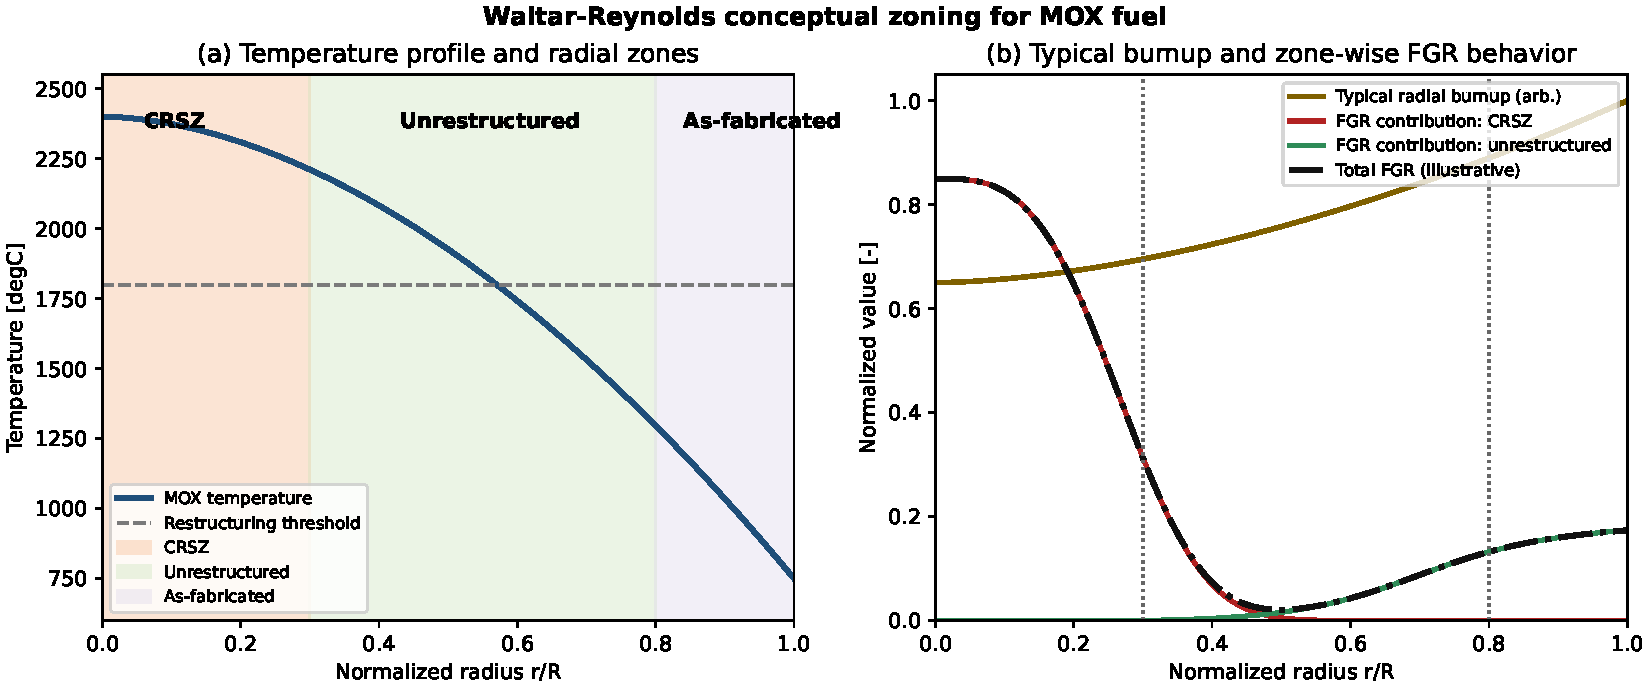
\includegraphics[width=0.98\textwidth]{images/waltar_reynolds_zones.pdf}
  \caption{Illustrative Waltar-Reynolds interpretation for MOX fuel: (a) a
  steep radial temperature profile and corresponding conceptual zone partition
  (CRSZ, unrestructured, and as-fabricated outer region); (b) representative
  zone-wise FGR behavior versus radius with a typical radial burnup profile.
  This figure is schematic and intended to clarify model logic, not to provide
  calibrated prediction data.}
  \label{fig:waltar_reynolds_zones}
\end{figure}

For each layer, the fractional area in each zone is evaluated from the radial temperature profile and the release fraction is area-averaged.  The global release ODE is:

\begin{equation}
  \frac{d\mu_{rel}}{dt}
  = \sum_j \frac{d\mu_{gen,j}}{dt} \cdot \overline{\text{FGR}}_j
  \label{eq:fgrel_ode}
\end{equation}

% -------------------------------------
\subsection{Internal Gas Pressure}
\label{sec:gpres}
% -------------------------------------

The internal gas pressure is determined by the ideal gas law applied to all void volumes:

\begin{equation}
  p_{gas} = \frac{(\mu_0 + \mu_{rel})\,R}{V_t}\times10^{-6}
  \quad \text{[MPa]}
  \label{eq:gpres}
\end{equation}

where $\mu_0$ [mol] is the initial fill-gas inventory, $R = 8.314$\,J/(mol\,K) is the universal gas constant, and the effective void volume at temperature is:

\begin{equation}
  V_t = \frac{V_{plenum}}{T_{pl}}
        + \sum_j \frac{\pi\,\Delta z_j\,(r_{ci,j}^2 - r_{fo,j}^2)}{T_{gap,j}}
        + \sum_j \frac{\pi\,\Delta z_j\,r_{fi,j}^2}{T_{ctr,j}}
  \label{eq:vt}
\end{equation}

with $T_{gap,j}$ the mean gas temperature in the gap of layer $j$, $T_{ctr,j}$ the central hole temperature, and $r_{fi,j}$, $r_{fo,j}$, $r_{ci,j}$ the deformed radii.

% -------------------------------------
\subsection{Gap Conductance with Fission Gas Mixture}
\label{sec:gap_ox}
% -------------------------------------

As fission gas is released into the plenum and gap, the gas mixture thermal conductivity decreases because Xe and Kr are poor thermal conductors.  Using a geometric-mean mixing rule:

\begin{equation}
  h_{gap}^{OX} = h_{medium}^{mix(He,Kr,Xe)} + h_{rad} + h_{contact}
  \label{eq:hgap_ox_modular}
\end{equation}

The medium term is computed with the Ross-Stoute / Lanning-Hann rarefied-gas temperature-jump model \cite{lanning1975}:

\begin{equation}
  h_{gas} = \frac{k_{gas}}{\delta_{eff} + g_{jump}}
  \label{eq:h_gas}
\end{equation}

\begin{equation}
  g_{jump} = \frac{0.024688\,k_{gas}\,\sqrt{T_{avg}}\cdot 2}{p\,\alpha}
  \label{eq:gjump}
\end{equation}

where $\delta_{eff} = \max(\delta, \delta_{rough})$ and $\delta_{rough}=\sqrt{\rho_f^2 + \rho_c^2}$, with $\alpha = \max(0.01,\;0.425 - 2.3\times10^{-4}T_{avg})$ (clamped to 1000 K). This keeps the thermal block modular while allowing FRED-OX-specific gas chemistry.

\begin{equation}
  k_{mix} = k_{He}^{x_{He}/\Sigma}
             \cdot k_{Kr}^{x_{Kr}/\Sigma}
             \cdot k_{Xe}^{x_{Xe}/\Sigma}
  \label{eq:kmix}
\end{equation}

where the mole fractions are computed from the fill gas ($\mu_0$\,mol He) and the released fission gas (composition: 88.46\% Xe, 7.69\% Kr, 3.85\% He by Waltar \& Reynolds \cite{waltar1981}).  Individual gas conductivities:

\begin{align}
  k_{He}(T) &= 2.639\times10^{-3}\,T^{0.7085} \label{eq:k_he2}\\
  k_{Kr}(T) &= 8.247\times10^{-5}\,T^{0.8363} \label{eq:k_kr}\\
  k_{Xe}(T) &= 4.351\times10^{-5}\,T^{0.8618} \label{eq:k_xe}
\end{align}

The additional terms are:

\begin{equation}
  h_{rad} = \sigma_{SB}\,f_\varepsilon\,(T_f^2 + T_c^2)(T_f + T_c)
  \label{eq:h_rad}
\end{equation}

\begin{equation}
  f_\varepsilon = \frac{1}{1/\varepsilon_f + (r_{fo}/r_{ci})(1/\varepsilon_c - 1)}
  \label{eq:frad}
\end{equation}

\begin{equation}
  h_{contact} = \frac{33.3\,k_m\,(p_{fc} - p_{gas})}{H_c\,\sqrt{\delta_{rough}}}
  \label{eq:h_contact}
\end{equation}

% -------------------------------------
\subsection{Fuel Swelling (MATPRO Model)}
\label{sec:swelling}
% -------------------------------------

The MATPRO fuel swelling model \cite{hagrman1981} distinguishes solid-fission- product swelling (independent of temperature) and gaseous-bubble swelling (strongly temperature-dependent):

\begin{align}
  \dot{\varepsilon}^{sw}_{solid}
    &= 2.5\times10^{-29}\,\dot{F}
    \label{eq:swel_solid}\\
  \dot{\varepsilon}^{sw}_{gas}
    &= 8.8\times10^{-56}\,(2800-T)^{11.73}\,
       e^{-0.0162(2800-T)}\,e^{-8\times10^{-27}\,E_{dep}}\,\dot{F}
    \quad (T < 2800\,\text{K})
  \label{eq:swel_gas}
\end{align}

where $\dot{F}$ [fissions/(m$^3$\,s)] is the local fission rate and $E_{dep} = B\,\rho_{f,0}$ [J/m$^3$] is the total deposited fission energy. The isotropic volumetric swelling strain is $\dot{\varepsilon}^{sw} = f_{mult}(\dot{\varepsilon}^{sw}_{solid} + \dot{\varepsilon}^{sw}_{gas})$, where $f_{mult}$ is a user-defined swelling multiplier.

The swelling strain enters the Hooke's law as an inelastic (eigenstrain) contribution in each direction:

\begin{align}
  E(\varepsilon_\theta - \varepsilon^{th} - \varepsilon^{sw}/3)
    &= \sigma_\theta - \nu(\sigma_r + \sigma_z) \\
  E(\varepsilon_r     - \varepsilon^{th} - \varepsilon^{sw}/3)
    &= \sigma_r     - \nu(\sigma_\theta + \sigma_z) \\
  E(\varepsilon_z     - \varepsilon^{th} - \varepsilon^{sw}/3)
    &= \sigma_z     - \nu(\sigma_\theta + \sigma_r)
\end{align}

% -------------------------------------
\subsection{MOX Thermal Conductivity (Philipponneau 1992)}
\label{sec:mox_k}
% -------------------------------------

The Philipponneau model \cite{philipponneau1992} gives the as-fabricated MOX conductivity and is extended in FRED-OX to include burnup degradation:

\begin{equation}
  k(T) = \left(\frac{1}{a_c + 2.493\times10^{-4}\,T}
               + 88.4\times10^{-12}\,T^3\right)
         \frac{1 - p}{1 + 2p}
  \label{eq:k_mox}
\end{equation}

where $p = 1 - \rho/\rho_{th}$ is the porosity and the stoichiometry- and burnup-dependent coefficient is:

\begin{equation}
  a_c = 1.320\sqrt{(2 - x) + 0.0093} - 0.091
        + \frac{0.0038\,B}{9.33}
  \label{eq:ac_burnup}
\end{equation}

with $x$ the oxygen-to-metal ratio deviation from stoichiometry and $B$ the burnup in MWd/kgU.

% -------------------------------------
\subsection{Cladding: AIM1 Steel with Irradiation Creep}
\label{sec:aim1}
% -------------------------------------

The AIM1 austenitic steel thermal conductivity and heat capacity are based on the legacy FRED correlations (also implemented in Luzzi \cite{luzzi2004}):

\begin{align}
  k_{AIM1}(T) &= 13.95 + 1.163\times10^{-2}(T - 273.15) \quad \text{[W/(m\,K)]} \\
  c_{p,AIM1}(T) &= 431.0 + 0.177\,T + 8.72\times10^{-5}\,T^2 \quad \text{[J/(kg\,K)]}
\end{align}

Irradiation creep of AIM1 is modelled through an empirical creep rate function $\dot{\varepsilon}^{cr} = f(\sigma, T, \dot{F})$.  T91 ferritic-martensitic steel (no irradiation creep in the current implementation) uses the corresponding implemented correlations for $k$, $c_p$, Young's modulus and thermal expansion.

\printbibliography[heading=subbibliography,title={References}]
\end{refsection}

\clearpage

\begin{refsection}

\section{Metallic Fuel in Sodium (FRED-M-Na)}
\label{sec:fred_m_na}

FRED-M-Na extends the FRED platform for U-Pu-Zr ternary metallic fuel rods in sodium-cooled fast reactors.  The same core heat conduction and stress-strain equations (Section~\ref{sec:thermo_mech}) are used with HT-9 ferritic-martensitic cladding and additional physics specific to metallic fuel:

\begin{itemize}
\item \textbf{Ternary U-Pu-Zr phase diagram}: phase state (alpha, beta, gamma, delta) affects thermal properties.
\item \textbf{Thermal conductivity with Na infiltration and irradiation}: sodium filling of open pores increases effective conductivity; burnup further modifies it.
\item \textbf{Zirconium redistribution}: Zr migrates from the hot fuel centre to the cooler periphery under steep temperature gradients, changing composition and phase radially.
\item \textbf{Sodium infiltration}: sodium from the coolant infiltrates open fuel porosity after the fuel contacts the cladding.
\item \textbf{Fuel swelling (solid FP)}: solid fission product swelling narrows the gap on a per-at\% burnup basis.
\item \textbf{Fission gas release (Karahan empirical model)}: the cumulative release fraction $f_r$ is a burnup-saturation function calibrated to EBR-II data \cite{karahan2009}:
\begin{equation*}
  f_r(B_\mathrm{FIMA}) = 0.8\!\left(1 - e^{-100\,B_\mathrm{FIMA}/1.8}\right),
  \qquad \bar{B}_\mathrm{FIMA} \geq 8\times10^{-3},
\end{equation*}
where $100\,B_\mathrm{FIMA}$ converts to atomic percent and the condition enforces a rod-average burnup threshold of $0.8\,\mathrm{at\%}$ before any gas is released.  The fraction saturates near 80\,\% by ${\sim}10\,\mathrm{at\%}$; released Xe/Kr dilute the gap gas and raise plenum pressure.
\item \textbf{Cladding wastage}: lanthanides from fission products diffuse into HT-9, consuming cladding material.
\end{itemize}

All correlations are ported from the Fortran reference code \texttt{FRED\_M\_OCT24.SRC} \cite{timpanoFredM} following Karahan (2009) \cite{karahan2009}.

% -------------------------------------
\subsection{Time Integration: Fixed-Step Backward Euler with Explicit Irradiation-Physics Coupling}
\label{sec:mna_time_integration}
% -------------------------------------

FRED-ROD and FRED-OX advance the full DAE state vector $\mathbf{y}$ through SUNDIALS IDA's adaptive-step BDF corrector (Section~\ref{sec:sundials}). FRED-M-Na uses its own fixed-step driver instead, inherited from the structure of legacy \texttt{Baseir.for} and retained because attempts to drive the same physics through SUNDIALS IDA proved numerically fragile. The fission-gas swelling/contact transition produces a near-discontinuous change in residual character that causes IDA's adaptive step-size control to reduce $h$ to unacceptably small values, eventually exhausting the corrector's ability to converge, while the legacy fixed-step approach passes through the same regime without issue.  

Therefore, no IDA calls: \texttt{IDACreate}, \texttt{IDAInit}, \texttt{IDASolve}, or \texttt{IDAReInit} calls exist anywhere in the FRED-M-Na application. The SUNDIALS \texttt{N\_Vector} type is retained purely as a plain data buffer so that checkpoint and HDF5-restart machinery from \texttt{FredSolverBase} works without modification.

At each step two numerically distinct update steps are applied in sequence to two disjoint groups of state variables:
\begin{itemize}
\item an \textbf{implicit, backward-Euler} update for the primary thermal/mechanical DAE unknowns (temperatures, stresses and strains, gas pressure, fission-gas generation and release); and
\item an \textbf{explicit, forward-Euler} update for the irradiation-physics accumulators (burnup, GRSIS bubble/gas-release state, Zr redistribution, cladding wastage), evaluated \emph{after} the implicit solve.
\end{itemize}

Algorithm~\ref{alg:mna_timestep} summarises the complete per-step logic.

\begin{algorithm}[H]
\caption{FRED-M-Na: one fixed step $t_n \to t_{n+1} = t_n + \Delta t$}
\label{alg:mna_timestep}
\begin{algorithmic}[1]
  \Statex \textbf{--- Implicit backward-Euler solve ---}
  \For{outer $= 1$ \textbf{to} 60}
    \State Update $f_\mathrm{gen}$, $f_\mathrm{rel}$ by direct substitution
    \For{each axial layer $j = 1,\ldots,N_z$}
      \State Dense Newton solve ($\leq 25$ iters, FD Jacobian):
      \Statex \qquad\qquad solve for $[T_1,\ldots,T_{n_f+n_c},\;
                 \varepsilon^{sw}_i,\; \varepsilon^{cr}_i,\;
                 b,\; \boldsymbol{\sigma}, \boldsymbol{\varepsilon},\; P_\mathrm{gas}]$
      \Statex \qquad\qquad using $\dot{y}_k \approx (y_k - y_k^{(n)})/\Delta t$
                 for ODE rows, $\dot{y}_k = 0$ for AE rows
    \EndFor
    \If{$\|\Delta P_\mathrm{gas}\| < 10^{-6}$ \textbf{and} layer corrections $< 10^{-6}$}
      \State \textbf{break}
    \EndIf
  \EndFor
  \State Accept last current state even if residuals $> 10^{-6}$   (no SUNDIAL's style step-size shrink or retry)
  \Statex
  \Statex \textbf{--- Explicit forward-Euler update (\texttt{afterAcceptedStep}) ---}
  \For{each axial layer $j$}
    \State \textbf{Burnup}: $B_{FIMA,j} \mathrel{+}= \bigl(q_v''' \,/\, (E_{fiss}\,n_{HM})\bigr)\,\Delta t$
    \State \textbf{GRSIS} bubble/gas-release: explicit Euler sub-stepped at
           $\delta t \leq 1000\,\mathrm{s}$
    \State \textbf{Zr redistribution}: explicit Euler flux-difference, 20 sub-steps
    \State \textbf{Cladding wastage}: explicit Euler diffusion, 20 sub-steps
    \State \textbf{Gap state}: evaluate contact regime $\in \{\texttt{open},\; \texttt{soft},\; \texttt{closed}\}$ from updated gap geometry; update residual branch for next step
    \State \textbf{Hard-contact burnup}: on the first transition to \texttt{closed}, record $B_{FIMA,j}^{hard} \gets B_{FIMA,j}$ (used by the sodium-infiltration ramp-down, Eq.~\eqref{eq:sinf})
  \EndFor
  \State Sync updated irradiation state to residual assembler (one-step lag)
\end{algorithmic}
\end{algorithm}

\noindent\textbf{Performance.} A representative 2176-day base-irradiation simulation (\path{examples/fred_m_na/timpano_SAS_benchmark/base_irradiation/}) with $\Delta t = 1\,\mathrm{day}$ completes in approximately 80\,s wall-clock time on a single core.  Further optimisation of the integrator has therefore not been pursued.

\subsubsection{Implicit backward-Euler solve for the primary DAE unknowns}
\label{sec:mna_backward_euler}

At each fixed step from $t_n$ to $t_{n+1} = t_n + \Delta t$, every differential row of the DAE is discretised with the backward-Euler formula:
\begin{equation}
  \dot{y}_k \approx \frac{y_k(t_{n+1}) - y_k(t_n)}{\Delta t},
  \qquad \mathtt{id}_k = 1,
  \label{eq:mna_be}
\end{equation}
while algebraic rows ($\mathtt{id}_k = 0$) are left undifferentiated.  The \texttt{id}-array convention is identical to that passed to IDA by FRED-ROD and FRED-OX, so the per-layer irradiation ODEs ($b$, $\varepsilon^{sw}_i$, $\varepsilon^{cr}_i$) and the mechanical AEs are typed consistently across all three applications.  Unlike IDA, $\Delta t$ is fixed for the whole step --- there is no adaptive step-size control or local-truncation-error test.

The state vector is partitioned into three rod-scalar globals ($f_\mathrm{gen}$, $f_\mathrm{rel}$, $P_\mathrm{gas}$) and per-layer local blocks.  Layers couple only through the three globals, so the step is solved by an outer Picard sweep (Algorithm~\ref{alg:mna_timestep}, lines 1--8):
\begin{enumerate}
\item $f_\mathrm{gen}$ and $f_\mathrm{rel}$ are updated by direct substitution (their defining equations are explicit in those unknowns).
\item $P_\mathrm{gas}$ is solved \emph{jointly} with each layer's Newton block rather than by direct substitution, because its defining equation depends on all layers' current fuel/cladding radii and axial strain.
\item Each layer's block --- temperatures, per-layer irradiation ODEs ($b$, $\varepsilon^{sw}_i$, $\varepsilon^{cr}_i$), and mechanical AEs ($\boldsymbol{\sigma}$, $\boldsymbol{\varepsilon}$), plus the jointly-solved $P_\mathrm{gas}$ --- is solved by a dense Newton iteration (up to 25 steps, finite-difference Jacobian, tolerance $10^{-7}$) via Eq.~\eqref{eq:mna_be}.
\end{enumerate}
The sweep repeats until both the layer-Newton correction and the change in $P_\mathrm{gas}$ between sweeps fall below $10^{-6}$ (relative), capped at 60 outer iterations.  If the cap is reached, the current iterate is accepted as-is with no retry --- matching legacy \texttt{Baseir.for}'s \texttt{niter\,>\,1000 $\to$ goto\,100} escape.  In practice the sweep converges in 2--4 iterations throughout the full 2176-day benchmark, so this escape is never exercised.

\subsubsection{Explicit forward-Euler update for irradiation physics}
\label{sec:mna_forward_euler}

After the implicit solve has been accepted, \texttt{FredMNaSolver::afterAcceptedStep} advances the irradiation-physics accumulators using explicit (forward) Euler:
\begin{equation}
  X(t_{n+1}) = X(t_n) + \dot{X}\bigl(t_n,\,\mathbf{y}(t_n)\bigr)\,\Delta t,
  \label{eq:mna_fwd_euler}
\end{equation}
i.e.\ rates are evaluated at the already-accepted start-of-step state and not solved implicitly.  The four updated quantities are:
\begin{itemize}
\item \textbf{Burnup} ($B_{FIMA,j}$ per layer): $B_{FIMA,j} \mathrel{+}= (q_v''' / E_{fiss}\,n_{HM})\,\Delta t$.
\item \textbf{GRSIS bubble/gas-release state} (Section~\ref{sec:grsis}): the seven per-node concentrations ($c_{gfm}$, $c_{gb1}$, $c_{gb2}$, $c_{gb31}$, $c_{gb32}$, $c_{ggen}$, $c_{grel}$) are advanced as $X \mathrel{+}= \dot X\,\Delta t$, a direct port of legacy \texttt{GRSIS\_metalfuel.for}, which itself uses unguarded explicit Euler.  Because the legacy driver only called this routine with $\Delta t \approx 1000\,\mathrm{s}$, the call is internally sub-stepped to $\delta t \leq 1000\,\mathrm{s}$ to keep the explicit scheme in the stability regime the model was calibrated for.
\item \textbf{Zirconium redistribution} (Section~\ref{sec:zrdist}): the thermomigration diffusion equation~\eqref{eq:zrdist} is discretised by a conservative radial flux difference and advanced by forward Euler,
    \begin{equation}
      c_{Zr,i}(t+\delta t) = c_{Zr,i}(t) +
        \frac{2\,\delta t}{r_{i+1}^2 - r_i^2}
        \Bigl(r_i\,J_{i} - r_{i+1}\,J_{i+1}\Bigr),
      \label{eq:mna_zr_fwd_euler}
    \end{equation}
internally sub-stepped into 20 equal intervals $\delta t = \Delta t / 20$ (matching the legacy Fortran's count) for numerical stability against the diffusive term.
\item \textbf{Cladding wastage} (Section~\ref{sec:wastage}): the lanthanide diffusion/consumption model is likewise advanced by explicit Euler with 20 sub-steps per outer step.
\end{itemize}

None of these updates feed back into the Newton system for the \emph{same} step: their results enter the residual only at the \emph{next} step (one-step-lagged explicit coupling).  This mirrors the structure of legacy \texttt{Baseir.for}, which updates burnup, GRSIS, and Zr redistribution once per fixed step from the previous step's converged thermal/mechanical state.

\subsubsection{Gap-state detection without a root-finder}

FRED-ROD/FRED-OX locate gap contact-state transitions to machine precision via an IDA root function (Section~\ref{sec:gap_events}).  FRED-M-Na registers no root function --- with no adaptive integrator there is no continuous trajectory to search.  Instead, gap geometry and the \texttt{open}/\texttt{soft}/\texttt{clos} ratchet (Section~\ref{sec:upuzr_gap_states}) are re-evaluated once per fixed step in \texttt{afterAcceptedStep}, exactly as legacy FRED-M does.  A boundary-condition change detected this way needs no special re-initialisation because the one-step integrator carries no multistep history to invalidate.

% -------------------------------------
\subsection{U-Pu-Zr Phase Diagram}
\label{sec:phase}
% -------------------------------------

The ternary phase diagram is approximated by linear interpolation between binary U-Zr and U-19\%Pu-Zr boundaries (Karahan 2007, as was implemented in \texttt{Fphase.for} \cite{karahan2009}).  Six regions are identified by six temperature/composition boundary lines:

\begin{itemize}
\item $\alpha$: orthorhombic phase at low temperature and low Zr.
\item $\alpha + \delta$: two-phase region at intermediate Zr.
\item $\delta$: high-Zr phase.
\item $\beta$: body-centred cubic, intermediate temperature.
\item $\beta + \gamma$: two-phase BCC.
\item $\gamma$: high-temperature fully BCC; highest thermal conductivity.
\end{itemize}

The phase determines which thermal conductivity model is applied (see Section~\ref{sec:upuzr_k}).

% -------------------------------------
\subsection{U-Pu-Zr Thermal Conductivity}
\label{sec:upuzr_k}
% -------------------------------------

Three irradiated-fuel conductivity models are available, selectable at run time via \texttt{set\_conductivity\_model} (enum \texttt{ConductivityModel}); all three multiply the same fresh-fuel correlation $k_{fresh}$ by an irradiation correction and are evaluated per fuel node (node temperature and post-redistribution local composition; burnup is the layer value):

\begin{itemize}
\item \texttt{DetailedNaSodium} (default, \textbf{recommended}): irradiation-corrected conductivity with sodium infiltration.  Resolves the porosity state per node --- gas-filled versus sodium-logged pores --- combining the Maxwell-Eucken-type correction for sodium-filled porosity with the $(1-p)^{1.5}$ gas-porosity degradation.  The only model with an explicit physical mechanism for the conductivity recovery observed after sodium infiltration.
\item \texttt{EmpiricalBurnup}: piecewise burnup-only correction factor (Karahan 2009); no explicit porosity or sodium physics.
\item \texttt{SigmoidBurnup}: smooth sigmoid-fit burnup-only correction developed in the ESFR-SIMPLE project; a $C^\infty$ alternative to the piecewise empirical factor.
\end{itemize}

\subsubsection{Fresh Fuel (Aydin/Karahan 2009)}

The fresh-fuel conductivity is a quadratic function of temperature \cite{karahan2009}:

\begin{equation}
  k_{fresh}(T) = A + B\,T + C\,T^2 \quad \text{[W/(m\,K)]}
  \label{eq:k_upuzr}
\end{equation}

with composition-dependent coefficients:

\begin{align}
  A &= 17.5\left(\frac{1 - 2.23\,x_{Zr}}{1 + 1.61\,x_{Zr}} - 2.62\,x_{Pu}\right) \\
  B &= 1.54\times10^{-2}\,\frac{1 + 0.061\,x_{Zr}}{1 + 1.61\,x_{Zr}} \\
  C &= 9.38\times10^{-6}(1 - 2.7\,x_{Pu})
\end{align}

where $x_{Pu}$ and $x_{Zr}$ are the weight fractions of plutonium and zirconium.

\subsubsection{Irradiation-Corrected Conductivity (with Na Infiltration)}

During irradiation, two counteracting effects modify the thermal conductivity: fission product damage reduces $k$ while sodium infiltration into open pores increases it.  The Karahan model \cite{karahan2009} is:

\begin{equation}
  p_{Na} = f_{inf}\,(p_{tot} - p^{\text{clos}}_{gas}), \quad
  p^{\text{eff}}_{gas} = p^{\text{clos}}_{gas} + (p_{tot} - p^{\text{clos}}_{gas})(1 - f_{inf})
  \label{eq:pna}
\end{equation}

\begin{equation}
  P_c = 1 - \frac{3\,p_{Na}}{1 - p^{\text{eff}}_{gas}}\cdot
             \frac{1 - k_{Na}/k_U}{1.163 + 1.837\,k_{Na}/k_U}
  \label{eq:Pc}
\end{equation}

\begin{equation}
  k_{irr} = k_{fresh}\cdot P_c\cdot(1 - p^{\text{eff}}_{gas})^{1.5}
  \label{eq:k_irr}
\end{equation}

where $p_{tot}$ is the gas-bubble porosity ($= sw_{gas} = sw_{close} + sw_{open}$ from GRSIS, Section~\ref{sec:grsis}), $p^{\text{clos}}_{gas}$ the closed (gas-filled) porosity ($= sw_{close}$), and $p_{tot} - p^{\text{clos}}_{gas} = sw_{open}$ the open porosity accessible to sodium.  $f_{inf} \in [0,1]$ is the sodium infiltration fraction (Section~\ref{sec:sinf}): the fraction of the open porosity actually infiltrated by sodium, so $p_{Na}$ is the sodium-filled porosity and $p^{\text{eff}}_{gas}$ the effective gas porosity (gas-filled pores plus the un-infiltrated remainder of the open porosity).  $k_{Na}$ is the sodium thermal conductivity \cite{fink1995}.

\subsubsection{Empirical Burnup Correction (Karahan 2009)}

An alternative simplified correction as a function of burnup $B$ [at\%]:

\begin{equation}
  k_{corr} = \begin{cases}
    k_{fresh}\,\dfrac{1 - 0.135B}{1 + 1.7\times0.135B} & B \leq 2\,\text{at\%} \\[6pt]
    k_{fresh}\,(0.5 + 0.0667(B-2))                     & 2 < B \leq 5\,\text{at\%} \\[6pt]
    0.7\,k_{fresh}                                       & B > 5\,\text{at\%}
  \end{cases}
  \label{eq:k_bup_corr}
\end{equation}

\subsubsection{Sigmoid Burnup Correction (ESFR-SIMPLE)}

A smooth refit of the burnup degradation developed within the ESFR-SIMPLE project (legacy \texttt{Flamb.for}, \texttt{f=3}), expressed as the difference of two logistic functions of burnup $B$ [at\%]:

\begin{equation}
  k_{corr} = k_{fresh}\left[
    \frac{a_1}{1 + e^{-b_1 (B - c_1)}} -
    \frac{a_2}{1 + e^{-b_2 (B - c_2)}}
  \right]
  \label{eq:k_esfr}
\end{equation}

with fitted coefficients

\begin{center}
\begin{tabular}{lll}
  $a_1 = 100.27110592$ & $b_1 = 0.5474772$  & $c_1 = -8.15852445$ \\
  $a_2 = 99.62701$     & $b_2 = 0.64761187$ & $c_2 = -6.4644582$
\end{tabular}
\end{center}

The bracketed factor is ${\approx}1$ at $B = 0$, decreases smoothly with burnup, and saturates near $a_1 - a_2 \approx 0.64$ at high burnup.  It captures the same trend as Eq.~\eqref{eq:k_bup_corr} but is infinitely differentiable --- no slope discontinuities at 2 and 5\,at\% --- and does not reproduce the piecewise model's recovery from 0.5 back to 0.7 between 2 and 5\,at\%.

% -------------------------------------
\subsection{Sodium Infiltration}
\label{sec:sinf}
% -------------------------------------

The fuel is immersed in the sodium-bonded gap, so liquid sodium fills any interconnected fuel porosity it can reach. The sodium infiltration fraction $f_{inf}$ (code variable \texttt{psod}, a direct port of legacy \texttt{Sinf.for}) is modelled empirically as a function of burnup, radial position, fuel phase, and gap state \cite{karahan2009}:

\begin{equation}
  f_{inf} = \begin{cases}
    0 & \text{phase} \notin \{\alpha,\ \alpha{+}\delta\} \ \text{or}\ r < 0.6\,r_{fo} \\[4pt]
    0.6 & \text{gap state \texttt{open} or \texttt{soft}} \\[4pt]
    \max\!\bigl(0.3,\; 0.6 - 5\,(B_{FIMA} - B_{FIMA}^{hard})\bigr) & \text{gap state \texttt{clos}}
  \end{cases}
  \label{eq:sinf}
\end{equation}

where $r$ is the current node radius, $r_{fo}$ the outer fuel radius, $B_{FIMA}$ the local burnup, and $B_{FIMA}^{hard}$ the burnup at the moment of hard (full annular) fuel--cladding contact.  Infiltration is thus confined to the cooler outer 40\,\% of the fuel radius where the low-temperature $\alpha$ or $\alpha{+}\delta$ phase persists and porosity remains interconnected.  Once hard contact closes the gap, continued swelling squeezes sodium back out and $f_{inf}$ ramps down from 0.6 with burnup accumulated past hard contact, saturating at 0.3.  Sodium infiltration improves thermal conductivity (via Eq.~\eqref{eq:k_irr}).

% -------------------------------------
\subsection{Gap Conductance Specialization in FRED-M-Na}
\label{sec:gap_mna}
% -------------------------------------

FRED-M-Na uses the same platform thermal equation, but with an application- specific gap-conductance composition:

\begin{equation}
  h_{gap}^{M\text{-}Na} = h_{medium}^{gap\ material} + h_{contact}
  \label{eq:hgap_mna_modular}
\end{equation}

The no-jump medium closure is:

\begin{equation}
  h_{medium}^{M\text{-}Na} = \frac{k_{gap}(T_{avg})}{\delta_{eff}},
  \quad
  \delta_{eff} = \max\!\left(\delta,\sqrt{\rho_f^2+\rho_c^2}\right)
  \label{eq:hgap_mna_medium}
\end{equation}

The medium term is evaluated with a no-jump conductive closure (effective thermal gap width limited by roughness), while contact conductance is added in closed-gap states.

% -------------------------------------
\subsection{Zirconium Redistribution}
\label{sec:zrdist}
% -------------------------------------

A steep radial temperature gradient drives Zr diffusion from the hot fuel centre toward the cooler periphery.  The redistribution is governed by a thermomigration (Soret) diffusion equation:

\begin{equation}
  \frac{\partial x_{Zr}}{\partial t}
  = \frac{1}{r}\frac{\partial}{\partial r}
    \!\left(r\,D_{Zr}\left(\frac{\partial x_{Zr}}{\partial r}
    + \frac{x_{Zr}\,Q^*}{R\,T^2}\frac{\partial T}{\partial r}\right)\right)
  \label{eq:zrdist}
\end{equation}

where $D_{Zr}$ [m$^2$/s] is the diffusion coefficient, $Q^*$ [J/mol] the heat of transport, and $R$ the gas constant.  These parameters are phase-dependent (Karahan \cite{karahan2009}, from \texttt{Zrdist.for}).  The updated Zr profile changes the local thermal conductivity and phase state.

% -------------------------------------
\subsection{Fuel Swelling: Solid Fission Products}
\label{sec:upuzr_swelling}
% -------------------------------------

For metallic fuel the dominant swelling contribution early in life is from solid fission products.  Ogata (1999) \cite{ogata1999} gives a volumetric swelling rate of approximately 1.5\% per at\% burnup:

\begin{equation}
  \dot{\varepsilon}^{sw}_{vol} = 0.015 \cdot 100 \cdot \dot{B}_{FIMA}
  \label{eq:swel_metallic}
\end{equation}

where $\dot{B}_{FIMA}$ [FIMA/s] is the local fission-rate-based burnup rate per fissile atom.  For FRED-ROD/FRED-OX (and for FRED-M-Na in the \texttt{open} or \texttt{clos} gap-contact states, Section~\ref{sec:upuzr_gap_states}) the swelling enters the mechanics solver isotropically ($\varepsilon^{sw}/3$ per direction), in the same way as for MOX fuel (Section~\ref{sec:swelling}). In the \texttt{soft} contact state the partition is anisotropic instead — see Section~\ref{sec:upuzr_gap_states}.

% -------------------------------------
\subsection{Gap-Contact States and Anisotropic Swelling (open/soft/clos)}
\label{sec:upuzr_gap_states}
% -------------------------------------

Unlike FRED-ROD/FRED-OX's two-state (\texttt{open}/\texttt{closed}) gap model (detected by a SUNDIALS IDA root, shared platform mechanism), U-Pu-Zr metallic fuel's anisotropic axial swelling produces localized fuel-clad contact well before the bulk annular gap geometrically closes. FRED-M-Na therefore tracks a third, intermediate contact state, \texttt{soft}, matching legacy FRED-M's \texttt{Baseir.for}/\texttt{Fanis.for} model. The state is a monotonic ratchet for U-Pu-Zr fuel (\texttt{open} $\to$ \texttt{soft} $\to$ \texttt{clos}, never reverses), detected once per accepted fixed step by checking gap geometry directly (no root-finder --- FRED-M-Na does not use SUNDIALS IDA at all, see Section~\ref{sec:mna_time_integration}), rather than at an exact root-crossing time as FRED-ROD/FRED-OX do:

\begin{equation}
  \text{flag} = \begin{cases}
    \texttt{open} & r_{ci} - r_{fo} > \delta_{ruff} \\
    \texttt{soft} & r_{ci} - r_{loc} \le \delta_{ruff},\ \ r_{loc} = r_{fo} + f_{anis}\,g_0 \\
    \texttt{clos} & r_{ci} - r_{fo} \le \delta_{ruff}
  \end{cases}
  \label{eq:gap_flag}
\end{equation}

where $f_{anis}$ is the fuel axial anisotropy factor (Fanis.for, function of linear power and Pu content) and $g_0$ the as-fabricated gap. Once \texttt{soft} or \texttt{clos} is reached the local swelling partition switches from isotropic to anisotropic (radial/hoop only, axial suppressed), reflecting that new swelling is redirected into the still-open radial direction rather than axial elongation once localized contact constrains the fuel axially:

\begin{equation}
  \Delta\varepsilon^{sw}_z, \Delta\varepsilon^{sw}_h, \Delta\varepsilon^{sw}_r =
  \begin{cases}
    \left(\max(0,\tfrac{\Delta\varepsilon^{sw}_{vol}}{3}),\ \max(0,\tfrac{\Delta\varepsilon^{sw}_{vol}}{3}),\ \max(0,\tfrac{\Delta\varepsilon^{sw}_{vol}}{3})\right) & \text{open, clos} \\
    \left(0,\ 0.4995\,\Delta\varepsilon^{sw}_{vol},\ 0.4995\,\Delta\varepsilon^{sw}_{vol}\right) & \text{soft}
  \end{cases}
  \label{eq:swel_anisotropy}
\end{equation}

(the $0.4995$ coefficients sum to $0.999$, not $1.0$ — an intentional $\sim0.1\%$ volume loss/roundoff already present in the legacy Fortran). The flag also selects the mechanical boundary-condition branch at four locations (fuel axial force balance, fuel outer radial BC, cladding axial/interface BC, cladding inner radial BC); \texttt{soft} behaves like \texttt{clos} at the first three (shared axial load / strain continuity) but like \texttt{open} at the cladding inner radial BC, since contact is localized rather than full annular and the fill gas still surrounds the cladding ID. This three-state mechanics is implemented entirely in the FRED-M-Na application layer (a composition-based fork of the shared \texttt{StressStrain} residual class) so it has no effect on FRED-ROD/FRED-OX, which keep the shared two-state model unchanged.

% -------------------------------------
\subsection{GRSIS Fission-Gas Bubble Swelling Model}
\label{sec:grsis}
% -------------------------------------

The gaseous swelling and gas release of U-Pu-Zr fuel are computed per fuel
node by the GRSIS model (Lee 1999, as calibrated in Karahan 2009
\cite{karahan2009}; direct port of \texttt{GRSIS\_metalfuel.for} into
\texttt{FredMNaGrsis.hpp}).  The fission gas at each node is partitioned
into five populations plus two bookkeeping totals:

\begin{center}
\begin{tabular}{ll}
\toprule
$c_{gfm}$          & gas atoms dissolved in the fuel matrix [atom/m$^3$] \\
$c_{gb1},\,c_{gb2}$  & gas in \emph{closed} small / large bubbles \\
$c_{gb31},\,c_{gb32}$& gas in \emph{open} small / large bubbles \\
$c_{ggen},\,c_{grel}$& cumulative generated / released gas \\
\bottomrule
\end{tabular}
\end{center}

\subsubsection{Gas equation of state and bubble kinetics}

Gas is generated at $\dot c_{ggen} = 0.25\,\dot F$ (0.25 stable gas atoms
per fission, $\dot F$ the fission rate density).  The gas content of a
bubble of radius $r_i$ and volume $v_{bi}$ follows a capillarity equation of
state with a dense-gas volume floor:

\begin{equation}
  \rho_{gi} = \frac{v_{bi}}{\dfrac{k_B T}{2\gamma/r_i + \sigma_h} + \Omega},
  \qquad \sigma_h = p_{gas} + 2\,\mathrm{MPa},
  \quad \Omega = 85\times10^{-30}\,\mathrm{m^3},
  \label{eq:grsis_eos}
\end{equation}

giving atoms per bubble ($\gamma$ = surface tension); bubble number
densities follow as $n_i = c_{gbi}/\rho_{gi}$.  Gas-atom diffusion is
Arrhenius, $D_g = D_{g0}\exp(-Q_g/RT)$, and drives four capture fluxes and
a nucleation term:

\begin{equation}
  j_{gi} = \epsilon_i\, 4\pi r_i D_g\, c_{gfm}\, n_i, \qquad
  j_{nucl} = k_{nucl}\, c_{gfm}\, \rho_{g1},
  \label{eq:grsis_capture}
\end{equation}

so the matrix balance is $\dot c_{gfm} = \dot c_{ggen} - \sum_i j_{gi} -
j_{nucl}$.  Closed bubbles migrate by surface diffusion with mobility
$D_{bi} = 1500\,a^2 D_g / (\pi r_i^4)$ ($a$ = area per surface molecule)
and coalesce through binary collision kernels
$k_{ij} = \epsilon\,4\pi(r_i{+}r_j)(D_{bi}{+}D_{bj})$; a second coalescence
channel comes from radial growth, using the mean inter-bubble spacing
$\ell_i = 1.122\,n_i^{-1/3}$ and growth rates
$\dot r_i = j_{gi} r_i/(3 c_{gbi})$.  These terms assemble the four bubble
population balances $\dot c_{gb1}$, $\dot c_{gb2}$, $\dot c_{gb31}$,
$\dot c_{gb32}$ (small bubbles feed large ones; closed bubbles feed open
ones).

\subsubsection{Interconnection, release, and swelling}

When the closed-bubble swelling reaches the interconnection threshold
$sw_{close} \geq s_{th}$, a fraction $f_{th}$ of the closed-bubble gas
converts to the open populations per step.  All gas arriving in open
bubbles — by capture, coalescence, or conversion — is counted as released
to the plenum ($c_{grel}$), where it feeds the rod gas pressure and gap-gas
dilution.  The swelling components are

\begin{equation}
  sw_{close} = \sum_{i=1,2} \frac{c_{gbi}}{\rho_{gi}} v_{bi}, \qquad
  sw_{sol} = 0.015 \times 100\,B_{FIMA}, \qquad
  sw_{tot} = \max(sw_{sol} + sw_{close} + sw_{open},\ sw_{tot}^{prev}),
  \label{eq:grsis_swelling}
\end{equation}

with $sw_{sol}$ the solid-FP contribution (1.5\,\% per at\%) and $sw_{tot}$
constrained monotonically non-decreasing.  The open-bubble swelling
$sw_{open}$ is additionally subject to \textbf{hot pressing} once the gap is
closed: a creep-driven densification rate evaluated at the equivalent
stress $\sigma_{eq} = 3\sqrt{3\alpha_c}\,\min(p_{gas}, p_{fc})$, with
$\alpha_c = \tfrac16 \min(sw_{open}/0.1,\,1)^{1.5}$, reduces $sw_{open}$
each step (capped at $1.5\,\Delta B_{FIMA}$).

\subsubsection{Parameter presets and coupling}

Two calibration presets are selectable via \texttt{set\_grsis\_data\_mode}
(Section~\ref{sec:mna_time_integration}):

\begin{center}
\begin{tabular}{lcc}
\toprule
 & \texttt{FEAST} (default) & \texttt{GRSIS} (Lee 1999) \\
\midrule
$r_{b1},\,r_{b2}$ [µm]      & 0.5, 10  & 0.5, 12.5 \\
$\gamma$ [N/m]               & 0.8      & 1.0 \\
$D_{g0}$ [m$^2$/s], $Q_g$ [cal/mol] & $2.3\times10^{-3}$, 52000 & $0.95\times10^{-8}$, 32000 \\
$s_{th},\,f_{th}$            & 0.1, 0.01 & 0.2, 0.3 \\
\bottomrule
\end{tabular}
\end{center}

GRSIS couples back into the rest of FRED-M-Na through three paths:
(1)~$\mathrm{d}(sw_{tot})/3$ drives the per-node volumetric swelling strain
$\varepsilon^{sw}$, hence gap closure and the contact ratchet;
(2)~released gas $c_{grel}$ feeds the plenum pressure and gap-gas mixture;
(3)~the per-node bubble state sets the porosity seen by the detailed
Na-infiltration conductivity model (Section~\ref{sec:upuzr_k}) using
GRSIS's own split, identical to legacy \texttt{Baseir.for}:
$p_{tot} = fr_{tot} = sw_{gas}$ and
$p^{\text{clos}}_{gas} = fr_g = sw_{close}$, so the open porosity that
sodium can infiltrate is exactly $sw_{open}$.  Because surviving open
porosity peaks at intermediate temperatures — the hot centre closes its
open bubbles by hot pressing, while the cool periphery grows few — the
gas-porosity knock-down of the fuel conductivity is strongest at
mid-radius, not at the centreline (and is relieved further out where the
$\alpha$-phase sodium gate opens).

% -------------------------------------
\subsection{Fission Gas Release (Karahan Empirical Model)}
\label{sec:upuzr_fgr}
% -------------------------------------

The empirical FGR fraction for U-Pu-Zr (Karahan 2009 \cite{karahan2009}, from \texttt{FGR.for}) is a function of the average fuel burnup $\bar{B}_{FIMA}$ [at\%]:

\begin{equation}
  \text{FGR} = \begin{cases}
    0                           & \bar{B}_{FIMA} < 0.8\,\text{at\%} \\
    f(\bar{B}_{FIMA})           & 0.8 \leq \bar{B}_{FIMA} \leq 10\,\text{at\%}
  \end{cases}
  \label{eq:fgr_metallic}
\end{equation}

The threshold of 0.8\,at\% corresponds to the burnup at which the fuel first contacts the cladding and gas communication with the plenum opens.

% -------------------------------------
\subsection{Cladding Wastage by Lanthanide Attack}
\label{sec:wastage}
% -------------------------------------

Lanthanide fission products (Ce, Nd, Pr, La) migrate from the fuel into the
HT-9 cladding, where they precipitate as intermetallic compounds that
consume cladding thickness.  Two models are selectable at run time via
\texttt{set\_cladding\_wastage\_model} (enum \texttt{CladWastageModel},
implemented in \texttt{FredMNaCladWastage.hpp}):

\begin{itemize}
\item \texttt{PrecipitationKinetics} (default): layer-lumped lanthanide
      inventory with a $\sqrt{D/t}$ precipitation-front law; direct port of
      \texttt{Clanth.for} \cite{timpanoFredM} with coefficients refitted to
      SAS4A/MFUEL simulations of ESFR-M pins.
\item \texttt{LaTracking}: per-fuel-node radial lanthanide diffusion
      following SAS4A/MFUEL (Theory Manual v5.7, App.~9.3); the wastage is
      the time-integrated lanthanide flux arriving at the fuel--cladding
      interface.  Physically more general (no geometry-specific refit).
\end{itemize}

In both models the wastage grows only while the gap is in \texttt{soft} or
\texttt{clos} contact (a solid transport path to the cladding exists), and
neither resets accumulated wastage: legacy \texttt{Clanth.for}'s
open-gap reset branch is unreachable for U-Pu-Zr because the gap-contact
ratchet never reopens (\texttt{Baseir.for}'s reopen check is gated
\texttt{fmat.ne.'upuzr'}).

\subsubsection{Precipitation-kinetics model}

The fuel-side lanthanide inventory builds up in proportion to the fission
energy deposited:

\begin{equation}
  \dot c_L = \frac{y_L\, q'''}{n_{tot}},
  \qquad y_L = 15.29\times10^{9}\ \mathrm{atoms/J},
  \label{eq:wastage_source}
\end{equation}

with $n_{tot}$ the fuel atom density.  Lanthanide transport into the
cladding is Arrhenius in the cladding inner-surface temperature $T_{ci}$
(floored at 800~K):

\begin{equation}
  D_L = D_{0L}\,\exp\!\left(-\frac{Q_L}{R\,T_{ci}}\right),
  \qquad D_{0L} = 1.633\times10^{6}\ \mathrm{m^2/s},
  \quad Q_L = 333\,962\ \mathrm{J/mol}.
  \label{eq:wastage_diff}
\end{equation}

While the gap is in \texttt{soft} or \texttt{clos} contact (a transport
path to the cladding exists), the wastage front advances by the
solubility-limited parabolic precipitation law:

\begin{equation}
  \frac{\mathrm{d}x_{wast}}{\mathrm{d}t}
  = \frac{1}{2}\,
    \frac{c_L - c_{sol}^{fuel}}{c_{sol}^{clad} - c_{sol}^{fuel}}
    \sqrt{\frac{D_L}{t}},
  \qquad c_{sol}^{fuel} = 0, \quad c_{sol}^{clad} = 0.1,
  \label{eq:wastage}
\end{equation}

i.e.\ lanthanides diffusing into HT-9 precipitate once the local
concentration exceeds the cladding solubility limit, giving the classic
$\sqrt{D_L t}$ front growth scaled by the fuel-to-cladding solubility
ratio ($c_{sol}^{fuel}$ from the Karahan thesis, $c_{sol}^{clad}$ from the
SAS4A manual normalised by the HT-9 number density).  The update is
advanced by explicit Euler with 20 internal sub-steps per accepted time
step (Section~\ref{sec:mna_time_integration}).  There is no explicit
neutron-fluence dependence — the irradiation driver enters only through
the lanthanide source term~\eqref{eq:wastage_source}.

\subsubsection{Lanthanide-tracking model (MFUEL)}

The \texttt{LaTracking} model resolves the lanthanide number density
$u(r,t)$ [\#/m$^3$] radially across the fuel, on the same vertex-centred
node grid as heat conduction:

\begin{equation}
  \frac{\partial u}{\partial t}
  = \frac{1}{r}\frac{\partial}{\partial r}
    \!\left(r\,D_{La}(T)\,\frac{\partial u}{\partial r}\right)
  + Y_{La}\,q''',
  \qquad
  D_{La} = D_{0}\exp\!\left(-\frac{Q_{0}}{R\,\max(T, T_{floor})}\right),
  \label{eq:la_diffusion}
\end{equation}

with the MFUEL App.~9.3 parameters $D_0 = 5.0$~m$^2$/s,
$Q_0 = 250$~kJ/mol, $T_{floor} = 800$~K (irradiation-enhanced diffusivity
floor), and the same yield $Y_{La}$ as
Eq.~\eqref{eq:wastage_source}.  Boundary conditions: symmetry at $r=0$;
at the fuel surface $r = r_{fo}$, zero flux while the gap is open, and a
Dirichlet sink $u(r_{fo}) = 0$ while in \texttt{soft}/\texttt{clos}
contact (lanthanides precipitate instantly on arrival at the cladding).
Numerically the sink is applied at the boundary \emph{face}, so the
surface half-cell keeps its fission source and drains through the final
face diffusivity — which is evaluated at the \emph{cladding inner
temperature} $T_{ci}$, making the cold cladding side rate-limiting for
lanthanide entry (interior nodes use their local fuel temperature).
The wastage depth integrates the arriving interface flux, normalised by
the cladding's lanthanide uptake capacity:

\begin{equation}
  \delta(t) = \frac{1}{u_{sol}} \int_0^t
              \left(-D_{La}\,\frac{\partial u}{\partial r}\right)_{r_{fo}}
              \mathrm{d}\tau,
  \qquad u_{sol}^{HT9} = 6.4\times10^{27}\ \mathrm{\#/m^3},
  \label{eq:la_wastage}
\end{equation}

implemented conservatively by inventory bookkeeping (absorbed = generated
$-$ $\Delta$inventory per sub-step), with the explicit scheme sub-stepped
to its diffusion stability limit.

\paragraph{Radial mesh requirement.}
The floored diffusivity makes the interface boundary layer very thin: the
penetration depth $\sqrt{2 D_{La} t}$ at $D_{La}(800\,\mathrm{K}) =
2.3\times10^{-16}$~m$^2$/s is only ${\sim}0.06$~mm 100 days after the sink
activates and ${\sim}0.27$~mm at end of life — thinner than a typical
thermal cell ($0.39$~mm at $n_f = 11$) for the entire irradiation.  The
sink flux is set by the concentration gradient across this layer, so a
solve on the thermal grid cannot resolve it and under-predicts the wastage
by ${\sim}45$\,\% (Fig.~\ref{fig:la_mesh}).  The diffusion equation is
therefore solved on a refined uniform radial subgrid of
$(n_f - 1)\times\texttt{la\_refine} + 1$ points with linearly interpolated
node temperatures.  The recommended (default) refinement is
\textbf{\texttt{la\_refine} = 8} fine cells per thermal cell
(${\approx}50$~µm spacing at $n_f = 11$), which is within 7\,\% of the
$\times16$ result at negligible cost; \texttt{set\_la\_subgrid\_refine}
changes it for convergence studies.  Convergence is slow
($\sqrt{\,}$-like, Fig.~\ref{fig:la_mesh}a) because the boundary layer
keeps sharpening as the bulk inventory grows.

\begin{figure}[htb]
  \centering
  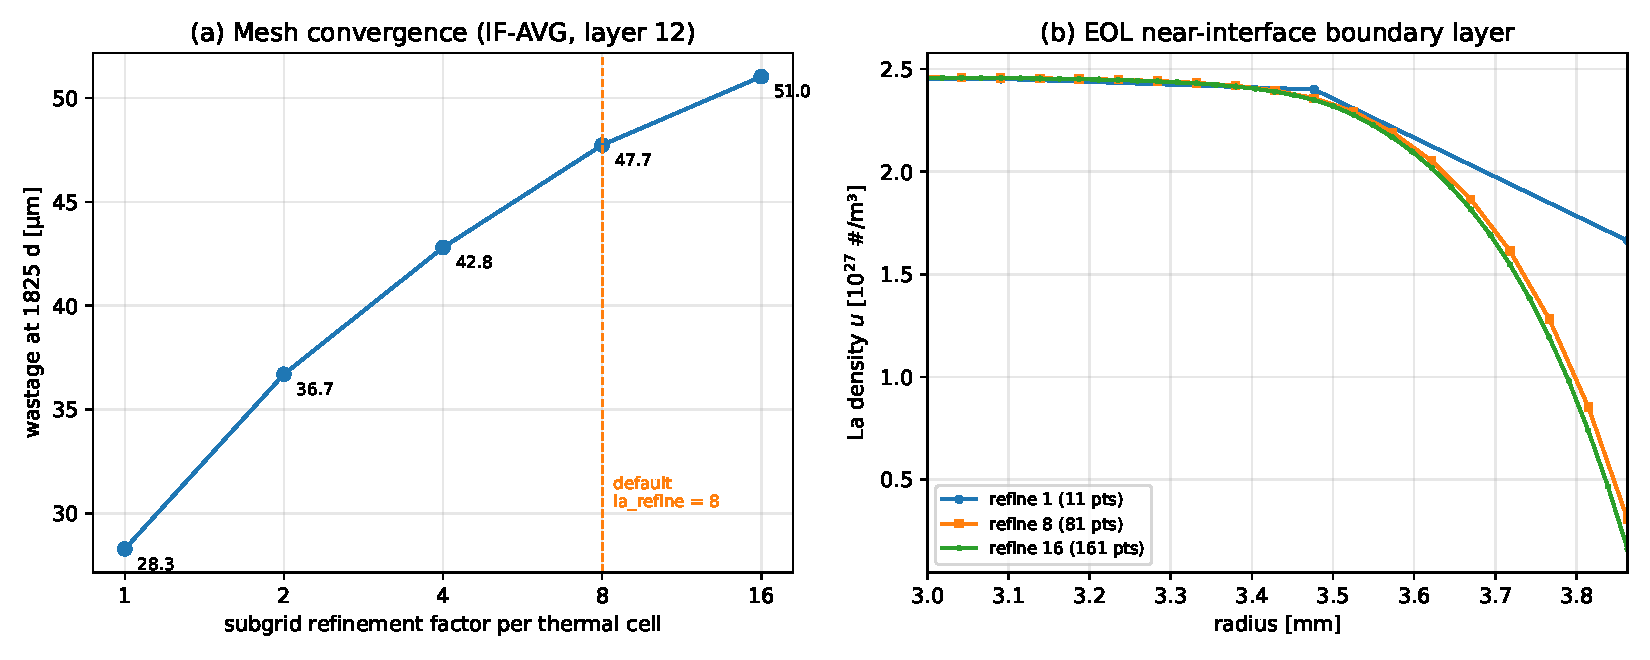
\includegraphics[width=0.95\textwidth]{images/la_mesh_refinement.pdf}
  \caption{LaTracking mesh-refinement study (IF-AVG benchmark, layer 12,
  1825~d): (a)~wastage vs.\ subgrid refinement factor per thermal cell —
  the thermal-grid solve (factor~1) recovers only 55\,\% of the
  $\times16$ reference, the default $\times8$ recovers 93\,\%;
  (b)~end-of-life lanthanide density near the fuel--cladding interface,
  showing the sub-cell boundary layer the coarse grid cannot represent.
  Generated by \texttt{images/make\_la\_mesh\_refinement.py}.}
  \label{fig:la_mesh}
\end{figure}

The contact gating of the sink is
selectable (\texttt{set\_la\_sink\_requires\_contact}): the default follows
the PK model's \texttt{soft}/\texttt{clos} gate, while the MFUEL-faithful
variant keeps the sink active from $t=0$ (transport through the sodium
bond).  The four-decade variation of $D_{La}$
between 800 and 1100~K makes the radial temperature profile the dominant
driver: the sink boundary layer stays confined to the cool outer
millimetre while the hot core remains source-dominated.  MFUEL declares
cladding failure at $\delta \geq 0.5\,t_{clad,0}$; FRED-M-Na streams the
per-layer $\delta$ (HDF5 \texttt{burnup/xwast\_layer}) and per-node $u$
(\texttt{burnup/c\_la}) for operating-limit assessment, with no feedback
onto the stress-strain solution.  See
\texttt{examples/fred\_m\_na/cladding\_wastage\_models/} for a
side-by-side comparison of the two models.

% -------------------------------------
\subsection{Cladding Void Swelling (HT-9)}
\label{sec:clad_swelling}
% -------------------------------------

Fast-neutron irradiation nucleates and grows voids in the HT-9 matrix,
producing a volumetric dilation of the cladding independent of thermal
expansion.  Two models are selectable at run time via
\texttt{set\_clad\_swelling\_model} (enum \texttt{CladSwellingModel},
implemented in \texttt{FredMNaCladSwelling.hpp}; \texttt{Cswel.for}'s
\texttt{icswel} flag in legacy) and are disabled by default (opt-in, since
this is new capability with no existing script depending on it):

\begin{itemize}
\item \texttt{Hofmann} (default): Hofmann (1985) void-swelling correlation
      \texttt{icswel=1}, a closed-form S-curve function of cumulative fast
      fluence, evaluated per clad node at that node's own temperature.
\item \texttt{SAS4A}: SAS4A User's Manual piecewise-linear swelling
      \emph{rate}, \texttt{icswel=2} (added Timpano/Daniele, 2024-08-06),
      gated on cladding dose and evaluated once at the cladding mid-wall
      temperature.
\end{itemize}

Both models consume the same SAS-derived fast-neutron fluence/dose
bookkeeping (\texttt{Baseir.for}):

\begin{equation}
  \dot{\phi} = q_l \, f_{ltpow} \times 10^{-26}\ \ [10^{22}\,\mathrm{n/cm^2/s}],
  \qquad q_l = q'''\,\pi\,(r_{fo0}^2 - r_{fi0}^2),
  \label{eq:sas_flux}
\end{equation}
\begin{equation}
  \nu(t) = \int_0^t \dot\phi\,\mathrm{d}\tau\ \ [10^{22}\,\mathrm{n/cm^2}],
  \qquad
  D_{dpa}(t) = \int_0^t \dot\phi\,D_{conv}\,\mathrm{d}\tau\ \ [\mathrm{dpa}],
  \label{eq:sas_dose}
\end{equation}

where $f_{ltpow}$ (fast-flux-to-linear-power ratio) and $D_{conv}$
(fluence$\to$dose conversion) are \emph{case-specific neutronics
calibration constants}, not universal physical constants: the defaults
($f_{ltpow} = 6.13209\times10^{14}$, $D_{conv} = 4.0$) are Timpano's
Serpent fit and SAS User's Manual value for the Inner-Fuel-Average pin
position (Superphenix-type spectrum) respectively, overridable via
\texttt{set\_fast\_flux\_calibration}.

\subsubsection{Hofmann (1985) void-swelling correlation}

\begin{equation}
  \frac{\Delta V}{V_0} = S_0 + D, \qquad
  S_0 = 0.01\,R\left[\nu + \frac{1}{\alpha}\ln\!
        \left(\frac{1+\exp[\alpha(\tau-\nu)]}{1+\exp(\alpha\tau)}\right)\right],
  \qquad
  D = (0.01)(0.15)\bigl[1-\exp(-0.10\,\nu)\bigr],
  \label{eq:hofmann_swelling}
\end{equation}
\begin{equation}
  R = 0.085\,\exp\!\left[-1\times10^{-4}(T_C - 400)^2\right],
  \qquad \alpha = 0.75,\quad \tau = 14.2,
  \label{eq:hofmann_R}
\end{equation}

with $T_C$ the clad node temperature in \textdegree C and $\nu$ the
cumulative fluence from Eq.~\eqref{eq:sas_dose} (in the same
$10^{22}$~n/cm$^2$ units the correlation was fit in --- note that, unlike
the historical Bison-manual fluence tracker retained in the output log for
reference only, both swelling models consume this one SAS-derived $\nu$).
$S_0$ is the void-formation term (a logistic incubation-then-growth curve
in fluence) and $D$ the solid-state-reaction term.  The linear (isotropic
$\Delta V/3$) strain applied per clad node is
$\varepsilon_{cs} = (\Delta V/V_0)/3$.

\subsubsection{SAS4A piecewise-linear model}

\begin{equation}
  \dot\varepsilon_{sw,HT9} = \begin{cases}
    0 & D_{dpa} < 100 \\[4pt]
    c(T)\;\dot\phi\,D_{conv} & D_{dpa} \geq 100
  \end{cases}
  \label{eq:sas_swelling}
\end{equation}

\begin{center}
\begin{tabular}{ll}
\toprule
$T$ range [K] & coefficient $c(T)$ [linear interpolation] \\
\midrule
$T \leq 673$        & $8.33\times10^{-5} \to 1.0\times10^{-4}$ \ (breakpoints 623/673) \\
$673 < T \leq 723$  & $1.0\times10^{-4} \to 8.33\times10^{-5}$ \\
$723 < T \leq 773$  & $8.33\times10^{-5} \to 5.0\times10^{-5}$ \\
$773 < T \leq 823$  & $7.5\times10^{-5} \to 2.5\times10^{-5}$ \\
$823 < T \leq 873$  & $5.0\times10^{-5} \to 1.25\times10^{-5}$ \\
$T > 873$           & $0$ \\
\bottomrule
\end{tabular}
\end{center}

evaluated at the cladding mid-wall temperature
$T_{mid} = \tfrac12(T_{ci} + T_{co})$ and integrated (explicit Euler) into
the isotropic linear strain
$\varepsilon_{cs} \mathrel{+}= \dot\varepsilon_{sw,HT9}/3 \cdot \Delta t$,
broadcast uniformly across all clad nodes (legacy: ``use midwall
temperature if model 2 is selected'').

\paragraph{The 100-dpa onset gate.} Void swelling in irradiated
ferritic-martensitic steels shows an experimentally observed
\emph{incubation dose}: at low damage, point defects (vacancies and
self-interstitials) generated by displacement cascades are efficiently
absorbed by the material's existing sink structure (dislocations,
lath/grain boundaries, precipitate interfaces) without net void
nucleation, so measured swelling is negligible.  Only once the dose
exceeds a threshold --- here 100 dpa, the SAS4A/HT-9 calibration --- does
the sink structure saturate and voids begin nucleating and growing at an
appreciable, roughly steady rate.  The SAS4A model represents this as a
hard step (zero below, piecewise-linear-in-$T$ above); the Hofmann
correlation instead builds the same incubation behaviour into a smooth
logistic term ($S_0$ above), which is why the two models can diverge
substantially in the first few hundred dpa even though both agree that
early-life swelling is negligible.

Neither model reduces $\varepsilon_{cs}$: void swelling is
irreversible, and (as with the wastage and GRSIS models) the gap-contact
ratchet never reopens for U-Pu-Zr, so there is no legacy reset branch to
reproduce here.  The isotropic strain $\varepsilon_{cs}$ is wired into
the clad Hooke's law identically to thermal expansion --- added with
coefficient $+1$ to the hoop, radial, and axial equations alike (unlike
creep, which is deviatoric and uses the standard $-1/+0.5/+0.5$ split).
FRED-M-Na streams $\varepsilon_{cs}$, $\nu$, and $D_{dpa}$ per layer/node
(HDF5 \texttt{swelling/ecs}, \texttt{swelling/neuflue2},
\texttt{swelling/dose}).  See
\texttt{examples/fred\_m\_na/cladding\_swelling\_models/} for a
side-by-side Hofmann-vs-SAS4A comparison validated against the legacy
Fortran reference.

% -------------------------------------
\subsection{HT-9 Cladding Material}
\label{sec:ht9}
% -------------------------------------

The HT-9 ferritic-martensitic steel correlations for thermal conductivity, heat capacity, thermal expansion, Young's modulus, and Poisson ratio are taken from Karahan (2009) \cite{karahan2009} and ported from \texttt{Clanth.for} in the reference Fortran code \cite{timpanoFredM}. No irradiation creep is currently modelled for HT-9.

% -------------------------------------
\subsection{Sodium Sub-Channel Coolant Model}
\label{sec:subchannel_mna}
% -------------------------------------

FRED-M-Na implements a one-dimensional sub-channel model to compute the local bulk coolant temperature and the cladding-to-coolant HTC axially from inlet conditions.  This enables the Robin boundary condition~\eqref{eq:robin_bc} to be applied without a separate T-H code. The last axial coolant temperature of the subchannel is also used to update the gas plenum temperature, which has a significant effect on the gas plenum pressure.

\subsubsection{Axial Coolant Energy Balance}

The coolant temperature rise from the rod inlet ($j=0$) to each axial layer $j$ is determined by a steady-state energy balance on the sub-channel control volume of layer $j$:

\begin{equation}
  \dot{m}\,c_{p,Na}(T_{co,j})\,\bigl(T_{co,j} - T_{co,j-1}\bigr)
  = q''_{co,j}\cdot 2\pi r_{co}\,\Delta z_j
  \label{eq:subchannel_energy}
\end{equation}

where
\begin{itemize}
\item $\dot{m}$ [kg/s] is the sub-channel mass flow rate,
\item $c_{p,Na}(T)$ [J/(kg\,K)] is the isobaric heat capacity of liquid sodium,
\item $T_{co,j}$ [K] is the bulk coolant temperature at the outlet of layer $j$ (inlet of layer $j+1$),
\item $q''_{co,j} = h_{cool,j}\,(T_{out,j} - T_{co,j})$ [W/m$^2$] is the cladding outer surface heat flux evaluated at the current outer cladding temperature $T_{out,j} \equiv T_{n_f+n_c-1,j}$, and
\item $\Delta z_j$ [m] is the layer height.
\end{itemize}

The equation is solved sequentially from $j=0$ to $j=n_z-1$, with $T_{co,-1} = T_{inlet}$ prescribed by the user.

\paragraph{Sodium thermophysical properties.} Liquid sodium density, specific heat, and thermal conductivity are evaluated from empirical correlations as functions of temperature. The sodium thermal conductivity is used internally for the gap conductance model (Section~\ref{sec:gap_mna}).

\subsubsection{Cladding-to-Coolant HTC Correlations}

The sub-channel HTC $h_{cool}$ [W/(m$^2$\,K)] is computed from a Nusselt number correlation for sodium-cooled pin bundles:
\begin{equation}
  h_{cool} = \frac{k_{Na}(T_{co})\,\mathrm{Nu}}{d_h}
  \label{eq:htc_def}
\end{equation}
where $k_{Na}$ is the sodium thermal conductivity, $\mathrm{Nu}$ the Nusselt number, and $d_h$ the hydraulic diameter of the sub-channel.

Two correlations are available.

\paragraph{Mikityuk (2009) correlation.}
\begin{equation}
  \mathrm{Nu}_{Mik} = 0.047\!\left(1 - e^{-3.8(P/D - 1)}\right)
                      \!\left(\mathrm{Pe}^{0.77} + 250\right)
  \label{eq:nu_mikityuk}
\end{equation}
valid for $1.1 \leq P/D \leq 1.95$ and $30 \leq \mathrm{Pe} \leq 5000$ \cite{mikityuk2009}, where $P/D$ is the pin pitch-to-diameter ratio and $\mathrm{Pe} = \mathrm{Re}\,\mathrm{Pr}$ the Péclet number.

\paragraph{Subbotin (Ushakov) correlation.}
\begin{equation}
  \mathrm{Nu}_{Sub} = 7.55\,\frac{P}{D} - 20\left(\frac{P}{D}\right)^{-13}
                      + \frac{3.67}{90}\,\mathrm{Pe}^{0.56 + 0.19\,P/D}
  \label{eq:nu_subbotin}
\end{equation}
\cite{subbotin1962}.  The Subbotin correlation was used in the legacy FRED-M reference code (option \texttt{COOL\_HTC 2}).

\paragraph{Péclet number.} The Péclet number for sodium flow is:
\begin{equation}
  \mathrm{Pe} = \frac{\dot{m}\,d_h}{A_{ch}\,\rho_{Na}}\,
                \frac{\rho_{Na}\,c_{p,Na}}{k_{Na}}
              = \frac{\dot{m}\,c_{p,Na}\,d_h}{A_{ch}\,k_{Na}}
  \label{eq:peclet}
\end{equation}
where $A_{ch}$ [m$^2$] is the sub-channel flow area.

\printbibliography[heading=subbibliography,title={References}]
\end{refsection}


% ===========================================================================
\end{document}
% ===========================================================================
